\documentclass[conference]{IEEEtran}

\usepackage[pdftex]{graphicx}
\usepackage[cmex10]{amsmath}
\usepackage{algorithmic}
\usepackage{caption}
\usepackage{subfig}
\usepackage{url}
\usepackage{balance}

\begin{document}
%\title{ What GitHub and Google Code can tell us about the Causes of Crashes of Android Apps? }
%\title{ A Mining Study the Google Code can tell us about the Causes of Crashes of Android Apps? }

%\title{What can the Issues of GitHub and Google Code tell us about Exception Fragilities in Android? }

%\title{What can the Issues of GitHub and Google Code tell us about Exception Fragilities in Android? }

%\title{Results of a Mining Study on Exception Stack Traces embedded on issues of over 600 Android Projects}

\title{Unveiling Robustness Threats by Mining the Exception Stack Traces of over 600 Android Projects}

%\title{Discovering Threats to Robustness through Exception Stack Trace Analysis: Results of a Mining Study of Android Projects}

%\title{Discovering Threats to Robustness through Exception Stack Trace Mining}

%\title{Discovering Threats to Robustness through Exception Stack Trace Mining of over 600 Android Projects}

%\title{Discovering Threats to Robustness through a Mining Study of Exception Stack Traces}

%\title{Discovering Fragilities on the Exception-Related Code through  Exception Stack Trace Mining}

%\title{On the Common Characteristics Android-Apps Crashes: Results of a GitHub and Google Code Mining Study}

%\title{On the Common Characteristics of Android-Apps Crashes: Results of a GitHub and Google Code Mining Study}

%\title{On the Common Characteristics of Android Crashes: Results of a GitHub and Google Code Mining Study}


%\title{A first Glance on Characteristics of Android Crashes: Results of a GitHub and Google Code Mining Study}


%\title{A first Glance on Characteristics of Android Crashes: Results of a GitHub and Google Code Mining Study}


\author{\IEEEauthorblockN{Roberta Coelho\IEEEauthorrefmark{1},
Lucas Almeida\IEEEauthorrefmark{1},
Georgios Gousios\IEEEauthorrefmark{2}, 
Arie van Deursen\IEEEauthorrefmark{2}
}
\IEEEauthorblockA{\IEEEauthorrefmark{1}Federal University of Rio Grande do Norte\\
Natal, Brazil\\
Email: \texttt{roberta@dimap.ufrn.br,lucas.almeida@ppgsc.ufrn.br}}
\IEEEauthorblockA{\IEEEauthorrefmark{2}Delft University of Technology\\
Delft, The Netherlands\\
Email: \texttt{\{g.gousios,arie.vandeursen\}@tudelft.nl}}
}

\newcommand{\todo}[1]{\textbf{TODO}\footnote{\textbf{TODO:} #1}}

% make the title area
\maketitle

%GitHub 315,92
% Google Code: 127,456
%All: 159,048


%The goal of this study was to: identify common characteristics 
%of such traces and investigate the fragilities on the exception-related code that can be revealed
%from them. 
%The goal of this study was to: identify common characteristics 
%of such traces and investigate the whether they can reveal
%the characteristics on the source code that may be favoring the introduction of faults 
%(i.e. Uncaught Exceptions, and Unintened handler Actions), and consequently
%decreasing the program robustness.
%(of apps or the underlaying framework) 



\begin{abstract}
The number of mobile apps is increasing in a daily rate. If on the one hand they
extend phones capabilities far beyond of the basic calls, on the other hand they have to 
cope with an increasing number of exceptinal conditions 
(e.g., faults in underlying middleware or hardware; memory and battery restrictions). 
Therefore, mechanisms for exception detection and handling are not an optional add-on but a 
fundamental part of such apps. However, studies have shown that such mechanisms are the less 
understood and tested parts of the system. As a consequence they may affect the system the 
other way around, making the system even less robust, leading to failures such as uncaught exceptions 
and unintended handling (i.e., exceptions being mistakenly caught by existing handlers).
This paper reports a study which mined the stack traces embedded on 
159,048 issues reported on Android projects hosted in GitHub (482 projs.) 
and Google Code (157 projs.). 
The goal of this study was to: investigate the whether the exception stack traces
 can reveal common characteristics on the exception-related code that
may be favoring the introduction of the aforementioned failures, which would be responsible for 
decreasing the application robustness. We call such characteristics ``fragilities" of the exception-related code.
Overall 6,005 exception stack traces were extracted, and analyzed in 
combination with source code and bytecode analysis. 
Some fragilities consistently detected in this study include: 
(1) undocumented runtime exceptions thrown by third party code;
(2) undocumented checked exceptions thrown by JNI native code;
(3) unexpected exception wrappings (e.g., Errors being wrapped in checked exceptions),
revealing that Java hybrid exception model is not fully used according to its purpose.
Moreover, about 50\% of all analyzed projects reported at least one NullPointerExeption
as the root cause of an exception stack trace.
This study provide important insights on how such fragilities impose challenges 
to application robustness not only in Android environment but also to other 
systems based on Java exception model.

\end{abstract}

%GitHub 31,592
% Google Code: 127,456
%All: 159,048



%\IEEEpeerreviewmaketitle

\section{Introduction}

Along the recent years, we have witnessed an astonishing increase in the number 
mobile applications. Such increase is motivated by pervasiveness of the World Wide Web 
and the unprecedented increase of global smartphone shipments -
the mobile industry shipped over 315 million smartphones in the last quarter of 2013 ~\cite{googleio}.

%the mobile industry shipped over 315 million smartphones in the last quarter of 2013
%The pervasiveness of the World Wide Web and the astonishing increase 
%in the number of smartphones stimulated the creation of applications which extend the phones
% capabilities far beyond of the basic calls and textual messages. 
%f we look at global smartphone shipments the numbers are astonishng;
%the mobile industry shipped over 315 million smartphones in the last quarter of 2013 [ref-googleIO].
%Such increase on smartphones combined with the pervasiveness of the World Wide Web
%have stimulated the creation of applications which extend the phones caVALIAR MOVER ESTE STACK TRACES PARA UMA FIGURA QUE MOSTR COMO ELE QUEBRADO... PELO EXCEPTION Mpabilities 
%far beyond of the basic calls and textual messages. 

In this context, Android has become a leading platform - thanks to its open-source 
model and hardware partners like Samsung, HTC, Motorola, Asus (besides Nexus Google's
 own device) ~\cite{gartner}.  Google estimates that there is over 1 billion Android active users per month ~\cite{googleio},
and the number of apps built on top of Android increases in a daily rate.

%ref: http://www.gartner.com/newsroom/id/2645115
% Gartner, Inc. Press release, 2012. www.gartner.com/newsroom/id/2237315.
% http://www.gartner.com/newsroom/id/2645115


%If on the one hand such applications are getting mode and more popular....
%On the other hand... there is a need for reliability, as some core functionalities 
%are moving to apps....such applications impose more challenges to software reliability 
%Such mobile platforms are intrinsically multi-threaded and support a development model 
% slightly (or sometimes drastically) different from those adopted on Web development [arie-icse],  
%abnormal computation states

%In the same rate the number of a users increase, also increases 
%the number of users affected by application faults and crashes.

If on the one hand such applications extend phones capabilities 
far beyond of the basic calls and textual messages, on the other hand
they have to face an increasing number of threats to application robustness
 arising from: faults in underlying middleware and hardware, 
faults on third party services and libraries; compatibility issues; 
faults on connected devices (e.g. camera, GPS); memory and 
battery restrictions; among others.

%Hence, in the same rate the number of mobile users increase, also increases 
%the number of users affected by such threats.
%faulty apps and app crashes.

Therefore, techniques for error detection and handling are not  an optional add-on but a 
fundamental part of such apps.
% as any other modern system~\cite{bruntink2006discovering}. 
The Android platform uses the exception handling mechanism embedded
 in Java to deal with such conditions. Although the exception handling mechanism
~\cite{goodenough1975exception} is one of the most used schemes for
detecting and recovering from such exceptional conditions, studies (e.g.~\cite{miller1997issues,Robil00,shah2010understanding, garcia2007extracting,garcia2001comparative,cabral2007exception,coelho2011unveiling}),
have shown that it is generally poorly understood and the less tested parts of the system ~\cite{coelho2011unveiling}.
As a consequence they may affect the system the other way around.
The exception-related code may favor the introduction of failures such as uncaught exceptions ~\cite{jo2004uncaught, zhang2012amplifying}
and unintended handling ~/cite{miller1997issues} (i.e., exceptions being mistakenly caught by existing handlers) 
which make the system even less robust.

% Google estimates that Android has over 1 billion active users per month, 
% who pull out theirs phones and check it over 100 billion times. 

%If we google for "Android app crashes"
% we can find 1.200.000 pages about the subject on forums and blogs. In Feb. 2014
%Gartner issue a report on mobile technologies and capabilities 
%[ref-https://www.gartner.com/doc/2665315/top--mobile-technologies-capabilities], 
%which emphasized the importance of monitoring application crashes.

Our conjecture is that several Android applications may be suffering from common 
fragilities on the exception-related code (of the applications themselves or 
the underlaying platform) which may be degratind the robustness of such applications.
We call ``fragilities" characteristics on the exception-related code that favor the introduction
of aforementioned failures.

%, and that such fragilities may be leading to
%decrease the application robustness, leading for instance to the Uncaught Exception problem -
% which is one of the main causes of application crashes ~\cite{jo2004uncaught, zhang2012amplifying}.
%investigate the whether the exception stack traces
% can reveal common characteristics on the exception-related code that
%may be favoring the introduction of the aforementioned failures, which would be responsible for 
%decreasing the application robustness. We call such characteristics ``fragilities" of the exception-related code.


%[ref AST].

In Java, when an application fails due to an uncaught exception, 
it automatically terminates, while the system prints a stack trace to the console, 
or log file ~\cite{gosling2000java}.  A typical Java stack trace consists of  the fully qualified name 
the thrown exception and the ordered list of methods that were active on the call stack before 
such exception has occurred ~\cite{gosling2000java,bloch2008effective}.

% The
%concentration of open source projects and the existence of initiatives that mine
%such information, such as GHTorrent~\cite{Gousi13}, allow the information about
%projects to be visible within and across projects and make a full population
%studies possible.

%Among the issues defined on issue trackers, we can find issues reporting bugs, and system crashes 
%found as a result of application executions. Such issues usually contain exception stack traces [ref][ref]. 
%<SUCH ISSUES INCLUDE STACK TRACES. WHAT IS THE RELATION BETWEEN STACK TRACE AND CRASH>
%<stack traces are part of good issues....>

%Stack traces are a useful source of information about system crashes, and is often used to support developers in debugging~\cite{schroter2010stack}. Moreover, information %from stack traces 
%combined with crash and bug reports can be used to support bug classification and clustering~\cite{wang2013improving, kim2011crash, %dhaliwal2011classifying}, fault-proneness prediction %models~\cite{kim2013predicting} and even automated bug fixing~\cite{sinha2009fault} tools. 

Until recent years, the availability of data, reporting such failures, was scarce. 
It comprised only few large scale projects (e.g. the Mozilla crash report dataset\footnote{https://code.google.com/p/promisedata/issues/detail?id=88}).
Recently we have observed a rapid increase in the number of open
source projects that make their version control systems as well as the issue tracking systems
publicly available in repository hosting sites such as GitHub and Google Code.

When available, the exception stack traces provide a useful source of information about system crashes ~\cite{bettenburg2008makes} which 
 can enable different kinds of post-mortem analysis and support:  debugging~\cite{schroter2010stack}, 
 bug classification and clustering ~\cite{wang2013improving, kim2011crash, dhaliwal2011classifying},  
automated bug fixing ~\cite{sinha2009fault} and fault-proneness prediction models ~\cite{kim2013predicting}. 

%Most of such studies, however, focused the analysis on one or two system at a time.
%This paper reports an exploratory study which targets a family of applications 
%(sharing the common Android framework) aiming at extracting 
%the common characteristics of exception stack traces reported to such systems to provide
%insights on similar fragilities on the exception related code of the applications and underlaying framework.

%482 applications) and Google code (157 applications)
%GitHub 31,592
% Google Code: 127,456
%All: 159,048

This study performs a post mortem analysis of the exception stack traces embedded on issues
reported on Android projects hosted in GitHub and Google Code. 
The goal of this study was to: investigate the whether the reported exception stack traces
 can reveal common fragilities on the exception-related code which may be favoring 
the introduction of failures such as uncaught exceptions - and as a consequence
 contributing to deacrease the robustness of apps.
To guide this investigation we compiled general guidelines on how to use
exceptions proposed by Gosling~\cite{gosling2000java},
Wirfs-Brock~\cite{wirfs2006toward} and Bloch~\cite{bloch2008effective}.
Then, using a custom tool called ExceptionMiner,
 which we develop specifically for this study, we mine stack traces from the issues reported 
on 482 Android projects hosted in GitHub and 157 projects hosted in Google Code.
Overall 159,048 issues were analyzed and 6,005 stack traces were extracted from them.
The exception stack trace analysis was augmented with additional information
extracted from JDK, Android Plaform and the applications using byte code 
and source code analysis. Manual inspection was used to leverage the understanding 
of exception stack traces and support further discussions and insights.

%projects: 788	 - projects with issues - 724 - 
%projects with issues (with exceptions): 243 
%projects with stacks: 158  -  stacks: 3559 (defect)
%Github: issues: 50342 - stacks: 3865 - projects: 2542 - projects with stacks: 293

%To guide our analysis, we compiled a set of best practices on how to use
%exceptions by composing relevant suggestions by Gosling~\cite{gosling2000java},
%Wirfs-Brock~\cite{wirfs2006toward} and Bloch~\cite{bloch2008effective}.  The
%comparison of those with the mined exceptions revealed several interesting
%findings, such as:

Some outcomes consistently detected during this study were the following:

\begin{itemize}

   \item  Unexpected exception wrappings (e.g., Error wrapping checked and runtime
    exceptions and vice-versa), indicating that the purpose of Java's hybrid exception model may not have been adequately used.

   \item Undocumented runtime exceptions signaled by third party code (i.e., libraries and Android platform). 
This study found 118 distinct methods defined on third party code and  reported as the root signalers of 
runtime exceptions. Only 1 of such methods (0,8\%) documented the explicitly thrown runtime exception 
in a Javadoc comment; and none of these methods included the exception as part of the exception 
interface (i.e., using throws clause).

   \item Undocumented checked exception signaled by native Android library. This finding points to a fragility 
on the way exceptions flow from JNI interface functions, which can lead to uncaught exceptions that are difficult do 
debug. 

  \item  A multitude of programming mistakes were reported as the main causes of exception stack traces:
 27,71\% of the analyzed exception stack traces reported a java.lang.NullPointerException the root cause;
and  51,96\% of all projects reported at least one exception stack trace on which the NullPoiterException
was the root cause.

\end{itemize}

As we can see, although the study was based on a subset of Android projects, 
the findings are not limited to this setting. The detected fragilities make difficult
or sometimes infeasible for a Java developer to prevent failures such as 
uncaught exceptions (e.g., thrown silently by third-party utility code), and 
unintended handling ( e.g., when an Error is wrapped in a checked Exception).
Thereore, they impose obstacles not only to the developement of robust Android apps, 
but also to the developement of any robust Java-based system. 
Hence, the study results are relevant to: (i) Android and 
Java developers to familiarize common characteristics and fragilities of exception-related code 
which is the first step to help developers preventing and dealing with them; and (ii) designers of languages and tools 
to consider ways of reducing such fragilities in Android and Java environments.
The main contributions of this study is twofold:
\begin{itemize}

  \item  It performs a large scale post morten analysis of exception stack traces reported on Android projects hosted in GitHub and Google Code.
  \item  It introduces ExceptionMiner, a tool developed to support exception stack trace mining and analysis.
    analysis.

\end{itemize}


% AVD: We have not looked at private issues, and the tool is described above.
%We strongly believe that, specially in the open-source environment,
%faults are not to be hidden in a private bug issue. Faults should be shared and
%discussed, so that a developer can learn from other projects mistakes.
%Currently, the search facilities of repositories are very limited, and the
%ExceptionMiner tool is a contribution in this direction.

The remaining of this paper is organized as follows. Section 2 presents a
background on Android Platform and Java exception model. 
Section 3 presents the study design. Section 4 reports the study findings. 
Section 5 provides further discussions and insights.
Section 6 presents the threats to validity associated to this study. Finally Section
7 describes the related work, and Section 8 concludes the paper and outlines
directions for future work.

\section{Background}
\label{sec:back}

\subsection{The Android Platform} \label{sec:extypes}
Android is an open source platform for mobile devices based on Linux kernel,
which also comprises a subset of the core Java library, a set of third-party libraries (e.g.  SQLite),
the Dalvik runtime environment, and the Application Framework (which provides 
higher-level services to the applications running on the platform) ~\cite{andguide}.

%The Android platform is mostly implemented in Java and uses Java Native Invocation (JNI) to access native C/C++ code. 
%And as mentioned before, it reuses the embedded Java Exception model to detect and handle 
%abnormal computation states.

The Android Application Framework supports an event-driven development model. 
Among the basic elements that comprise an Android application, we can cite the
 Activity class. The Activity is the main class of an Android app (there is usualy one
Activity per application window). Each Activity defines a set of hook methods  
(e.g., OnCreate(), onPause()) that are dispatched automatically by the Android 
framework (by inversion of control), in response to infrastructure and application events.

The Android Application Framework also provides several supporting APIs, such as 
the APIs to support concurrent development (e.g. AsyncTask). 
Such APIs particularly useful due to the high demand for responsiveness 
in mobile environment (mobile apps can easily become 
unresponsive due to resource limitation and excessive network access).


%\begin{figure} \centering 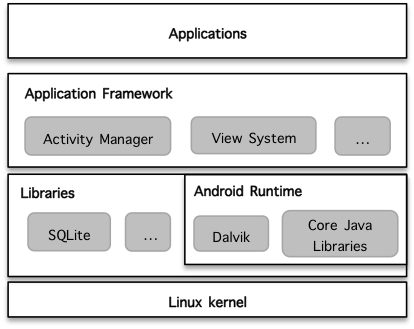
\includegraphics[scale=0.8]{arch3.png}
%  \caption{Android Architecture} \label{fig:exchier} \end{figure}

\subsection{Exception Model in Java} \label{sec:extypes}

In Java, an exception is represented according to the class hierarchy shown in
Figure~\ref{fig:exchier}.  According to it every exception is an
instance of the Throwable class, and can be of three kinds: the checked exceptions
(extends Exception), the runtime exceptions (extends RuntimeException) and errors
(extends Error)~\cite{gosling2000java}. The checked exception received such name
 because they must be declared on the method's exception interface (i.e., a list of exceptions that a method 
might raise during its execution) and the compiler statically checks if
 appropriate handlers are provided within the system.
Both runtime exceptions and errors are also known as unchecked exceptions, because 
they do not need to be specified on method exception interface and do not trigger any 
compile time checking.

By convention an Error represents an unrecoverable condition which usually results
from failures detected by the Java Virtual Machine, such as OutOfMemoryError and
normally should not be handled inside the application. The user-defined exceptions 
can be either checked or runtime. Although the Java specification~\cite{gosling2000java} 
suggests that user-defined exceptions should be checked exception (because doing so 
the callers of a method will know about the exceptions that a method can throw and so 
they can decide what to do about them) there is a long lasting debate about the use of 
checked and unchecked exceptions in Java. 

\begin{figure} \centering 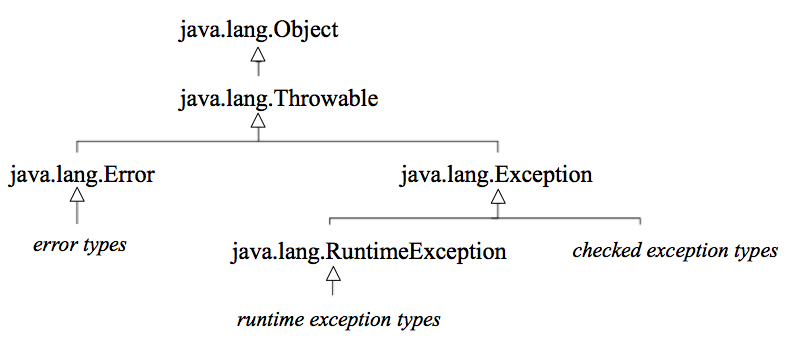
\includegraphics[width=\hsize]{new2_hierarchy.png}
  \caption{Exception Hierarchy in Java} \label{fig:exchier} \end{figure}

The runtime exceptions, however are not only used to represent user-defined
exceptional conditions, they are used by the JVM when a program violates 
the semantic constraints of the Java programming language (out-of-bounds array index, divide-by-zero 
error, null pointer references) from which most of the programs are not expected to recover. 
\footnote{Some programming languages react to such errors by peremptorily terminating the program; 
other programming languages allow similar approaches e.g.C\#; and others let the program to continue
 its execution in some situations such as the out-of-bounds array index e.g., C++. }

%In Java an exception can be thrown in one of the following
%circumstances~\cite{gosling2000java}: 
%(i) explicitly thrown when a throw statement is executed; 
%(ii) implicitly thrown by the JVM when the evaluation of an expression
% violates the normal semantics of language, also referred as a coding error
% (e.g., out-of-bounds array index, division-by-zero, access to a null reference); or 
%(iii) implicitly thrown by the JVM due to an internal error or resource limitation (e.g.,
%OutofMemoryError). 
%\todo{This sub-section is quite similar to the section introduction, shouldn't
%we merge them?}

%When an exception is thrown, it causes a transfer of control from the point
%where the exception occurred to a point that can be specified by the programmer
%(exception handler) - in Java it is represented by the try-catch block .

In Java, once an exception is thrown, the JVM looks for the nearest enclosing exception handler
(in Java it is represented by the try-catch block), and unwinds the execution stack if necessary.
 To look for the handler on the invocation stack is claimed to increase software reusability, 
since the invoker of an operation can handle it in a wider context ~/cite{miller1997issues}.


 A common way of  propagating exceptions in Java programs is through exception wrapping
 (also known as exception chaining). Exception wrapping allows one exception 
to be wrapped in another one and re-thrown. Figure~\ref{fig:wrapping} presents 
an exception stack trace which illustrates an exception wrapping. 
For simplicity we will refer to exception stack trace as stack trace along the text.
The bottom part of the stack trace is the \emph{root cause}, which indicates the
first reason for the error to be thrown (in this case, the computer run out of
memory). The top part of the stack trace indicates the location of the exception
manifestation (which will call \emph{top level wrapper} along this paper). The
execution flow  between the root cause and the exception manifestation may
include other intermediate exception wrappings. In all levels, the exception
\emph{signaler}, is the method that threw the exception, represented on the
stack trace as the first method call below the exception declaration.

\begin{figure} \centering 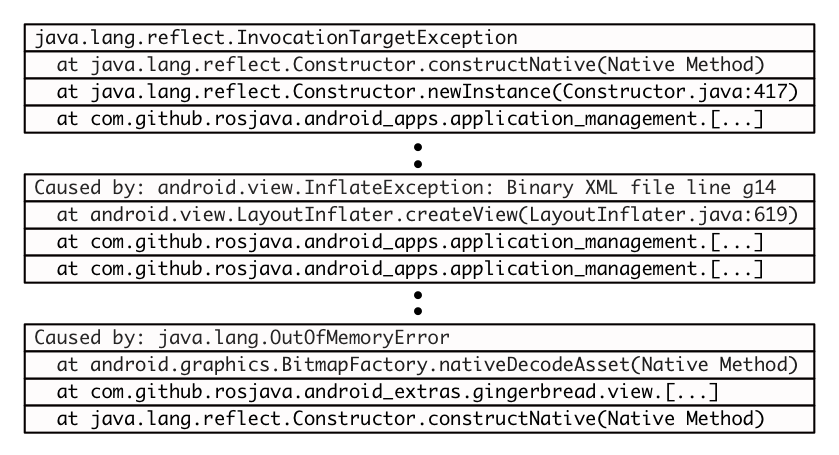
\includegraphics[scale=0.6]{stacktrace_bw.png}
\caption{Example of an exception stack trace in Java.}
\label{fig:wrapping}
\end{figure}

%<AVALIAR MOVER ESTE STACK TRACES PARA UMA FIGURA QUE MOSTR COMO ELE É QUEBRADO...
%PELO EXCEPTION MINER E AS INFORMAÇÕES VAO PARA O BANCO...>

% \subsection{Public Project Repositories and Issue Trackers} 
% ONE OF THE REVIEWERS COMPLAINED ABOUT THE ABSENCE OF EXPLANATIONS OF WHAT AN ISSU IS...
% As mentioned before, currently more and more projects are becoming available in 
% public project repositories such as GitHub and Google Code.
% Such repositories provides facilities such as....
% The issue trackers available in such projects ....

\subsection{Best Practices}
\label{sec:best}

There is a long-lasting debate about the pros and cons of checked and unchecked exceptions 
~\cite{javatut,stackoverlow,debate},\footnote{152 questions in Stackoverlow
are related to this debate}. Such debates, however, are mainly based on the developers own experience in
using both approaches - since there is a lack of empirical studies on their the pros and cons.

Nevertheless, several general guidelines have been proposed on how to use Java
exceptions~\cite{mandrioli1992advances,gosling2000java,wirfs2006toward,
bloch2008effective}. Such guidelines do not focus on 
advocating any specific exception type, but rather propose ways to effectively use each of them.
 We compiled a list of the guidelines related to exception types in Java, 
summarized below:\footnote{We also compiled guidelines related
to exception handling but they are out of the scope of this paper.}

%\noindent\emph{Meaning of Exception Types}

%\textbf{I
\emph{I-Checked exceptions should be used to represent recoverable
conditions} (\cite{mandrioli1992advances,gosling2000java,wirfs2006toward,bloch2008effective})
The developer should use checked exceptions for conditions from which the caller
is expected to recover. By confronting the API user with a checked exception,
the API designer is forcing the client to handle the exceptional condition. The
client can explicitly ignore the exception (swallowing, or converting it to
other type) at the expense of the program's robustness~\cite{gosling2000java}.

\emph{II-Error represents an unrecoverable condition detected by the JVM which
should not he handled} (\cite{gosling2000java}). It results from failures detected
by the Java Virtual Machine which indicate resource deficiencies, invariant
failures or other conditions that make impossible the program to recover.

%\noindent\emph{Exception Throwing}

\emph{III-A method should throw exceptions that precisely define the
exceptional condition} (\cite{gosling2000java,bloch2008effective}). To do so,
developers should either try to reuse the exception types already defined in the
JVM or they should create a specific exception. Throwing general types such as a
pure java.lang.Exception or a java.lang.RuntimeException is considered a bad practice.

%\textbf{IV-Do not repeatedly re-throw exceptions, handle exceptions as close as
%possible to the problem}~\cite{wirfs2006toward}. 
%Programs that frequently throw exceptions lose in performance ~\cite{wirfs2006toward,gosling2000java}.
%Moreover, 
%Close to the place that the exception was throw the caller usually has
%enough contextual information to perform  corrective actions. When the exception
%is propagated far away from the method where it was signaled (i.e. further away
%#from the problem) it can be difficult to take meaningful recovery actions.
%*~\todo{RSC:this practice was not well explored, can be removed if we need space.}

%\noindent\emph{Exception Documentation}
%\textbf{IV- It is wise to document all exceptions thrown by a method} 

\emph{IV- All exceptions explicitly thrown by a method should be documented.}
(\cite{mandrioli1992advances,gosling2000java,wirfs2006toward,bloch2008effective}).
The exceptions thrown by a method are an important part of methods interface,
and is required to use the method properly. The checked exceptions are already
part of the  methods signature, and the method caller is aware of the checked
exceptions being thrown by it. According to~\cite{bloch2008effective}, it is
also wise to document the explicitly thrown runtime exceptions\footnote{This
excludes the implicitly signaled JVM runtime exceptions related to programming
mistakes} as carefully as checked exceptions. Doing so, the clients of a method
will be aware of all the exceptions the method can throw and can protect its code
against unforeseen exceptions. 

If the developer fails to do follow such practices (specially when developing 
library/reusable code) it will be difficult or even impossible for the caller to 
make effective use of such method~\cite{wirfs2006toward, bloch2008effective},
and protect the system against the uncaught exceptions - one of the main causes of 
systems crashes. 

These best practices guided our exploratory study described next.
Based on information extracted from stack traces (complemented by
bytecode and source-code analysis), we investigate whether stack characteristics
can reveal whether these practices have been obeyed.

%Next section discusses the
%study procedure and the practices' misuses that emerged from this study.


\section{Empirical Study Design}
\label{sec:study}

%This study focus on the analysis of crash information (related to uncaught exceptions) of a family of Android applications
%aiming at  extracting their common characteristics and looking for similar vulnerabilities on applications and underlaying platform.
%In Java when an application crashes due to an uncaught exception ... 
%Exception Stach trace is usually (procurar por artigo).

The goal of this mining study was to extract exception stack traces embedded on issues of Android projects 
(hosted in GitHub and Google Code), looking for its 
common characteristics and investigating whether
 they could reveal common fragilities on the exception code of both the 
applications and the underlaying  framework. 

Our study focused on open-source apps, since the information needed to perform our study
cannot be retrieved from commercial apps, whose issue reports and 
source code are not publicly available. The Android open-source apps were also 
target of other research studies ~\cite{Linar13,ahimed}.   

% Falar da assumption que stacj trá relacionada a crash?
%This study is built on the following assumption: the stack traces reported on issues contain 
%relevant information related to application crashes. Several studies and techniques have also based on this assumption %(e.g.,~\cite{sinha2009fault}~\cite{dhaliwal2011classifying}~\cite{kim2013predicting}).

%\subsection{Research Questions}
In the context of our study we formulated the following research questions:

\begin{description}

  \item[RQ1] \noindent\emph{What are the common characteristics of exception stack traces reported on issues?} 
Some of the common characteristics to be investigated are the exceptions reported as the root cause on
the exception stack trace, the origin of such exceptions (e.g., the application, a library, the Android platform). 

%Which fragilities on the exception-related code emerge from the exception stack trace analysis? 
%Can such characteristics reveal common fragilities on the exception code of applications or the underlying framework

%Which patterns of exception (mis)use emerge?
  \item[RQ2] \noindent\emph{Which fragilities on the exception-related code emerge from them?}
Based on a set of best practices compiled in this study, we investigated whether characteristics of exception stack traces  
can pinpoint best practices violations. Such  violations reveal fragilities
on the exception-related code, which threats the application dependability.

\end{description}

%Based mainly on the information available on exception stack traces embedded 
%on issues, the goal of this study was to gain a better understanding 
%of exception-related system crashes.

%Characteristics of exception stack traces and detected violations can reveal fragilities
% on the exception-related code, which threats the application dependability. 

For RQ1 and RQ2, we explore the domain quantitatively and highlight interesting cases by 
exploring cases qualitatively. To support this investigation, source code and bytecode 
analysis were used in combination with manual inspection to leverage the  understanding 
of stack traces and support further discussions and insights. 


\subsection{Data Extraction Process}
\label{sec:miningproc}

To answer the research questions the following information is needed: (i) the issues of reported on every Android project hosted on 
GitHub and Google Code; (ii) the stack traces embedded on those issues; (iii) the type of the exceptions
 reported on the stack traces (e.g., error, runtime, checked); (iv) the origin of such exceptions 
(e.g., the application, a library, the Android platform). Next sections describes how such information 
was retrieved from GitHub and Google Code, how the exceptions stack traces were extracted and distilled,
 and how the type associated to each exception and its origins was identified.

%mentioned 
%The data used in our study to answer our research questions are: the issues related to each 
%Android project available in each repository; the source code and manifest file of each application;
%the bytecode of all exceptions defined and reused by Android platform.

\subsubsection{Android Apps in GitHub}
\label{sec:git}

%As mentioned before, this study mined information available on GitHub issues,
%more specifically, extracting and distilling the stack traces embedded on GItHub issues. 

This study used the dataset provided by the GHTorrent project~\cite{Gousi13}, 
an off-line mirror of the data  offered through the Github API.  
To identify Android projects, we performed a case insensitive search for the
term \textsf{android} in the repository's names and short descriptions.  
Up to 23 Feb 2014,  when we queried GHTorrent, such heuristic could
 find 2.542 repositories,  from which 589 apps had at least one
issue containing a stack trace.

Then we performed further cleanup, inspecting the site of every Android
reporting at least one stack trace, to make sure that they represented real
mobile apps. During this clean up 106 apps were removed because they were either
example projects (i.e., toy projects) or tools to support Android development
(e.g. Selendroid, Roboeletric - tools to support the testing of Android apps).
The filtered set consisted of 482 apps. 

%4,208


%GitHub 31,592
% Google Code: 127,456
%All: 159,048

This set of 482 projects contained overall 31,592 issues from which 4,042 exception stack traces 
were extracted. Issues on Github are different from issues on dedicated bug tracking tools such as 
Bugzilla and Jira. The most important difference is that there are no predefined fields
  (e.g. severity and priority). Instead, Github uses a more open ended tagging system, on which
repositories are offered a pre-defined set of labels, but repository owners can modify 
them at will. Therefore, an issue may have none ore an arbitrary set of labels depending 
on which repository it was created. Table ~\ref{tab:lables} illustrates the ocurrences of different lables 
on the issues including exception stack traces.


% \centering
%  \begin{tabular}{|p{2cm}| p{5cm}|}
%    \hline



\begin{table}
  \centering
  \begin{tabular}{lr|lr}
    \hline
     \multicolumn{2}{c}{\bfseries{GitHub}} &  \multicolumn{2}{c}{\bfseries{Google Code}} \\
      \bfseries{Lable} &  \bfseries{\% Occurrences} &  \bfseries{Lable} &  \bfseries{\% Occurrences} \\
    \hline
empty &	54,24\% & Defect &	91,96\% \\
Defect &	39,56\%  & Enhancement  &	3,16\% \\
Enhancement &	0,57\% & Task	& 1,37\% \\
Support &	0,52\% & empty &	1,12\% \\
Problem &	0,36\% & StackTrace &	0,70\% \\
Others &	4,74\% &  Others &	1,68\% \\   
  \hline
  \end{tabular}
  \caption{Lables on issues including exception stack traces.}
  \label{tab:lables}
\end{table}

Based on the assumption that regardless the issue type, every exception stack
trace contains relevant information concerning the exception structure of the
projects analyzed - and therefore can review fragilities on the exception-related code -  
we opted for not restricting the analysis only on defect
issues.\footnote{We conducted the same analysis on the defect issues and the top
exceptions are similar to the ones mentioned on defect issues. Due to space
limitation we limit to present the general analysis here. More detailed analysis
on the defect issues can be found at:
\url{www.dimap.ufrn.br/~roberta/android_repo_mining}}

Moreover, issues and pull requests are dual on Github; all pull requests have a corresponding 
``backing'' issue which are automatically generated. Therefore, we excluded such automatically generated
issues from our analysis. Finally, the Github API allows the automated
generation of issues for specific repositories, which automated tools often use
to report crashes. In some cases, this led to high number of issues that
included stack traces. We identified and filtered those cases out (e.g.,
the~\textsf{pullwifi} project was responsible for almost 50\% of all Android issues in our dataset).

\subsubsection{Android Apps in Google Code}

Differently from GitHub, Google Code does not provide an API to access the information related
 to hosted projects \footnote{Google code used to provided a Web service to such repository, but it was deactivated in June 2013 what Google called a "clean-up action".}.

However, Google Code still contain largely used open-source Android apps (e.g. K9Mail \footnote{K9Mail moved to Github but as a way of not loosing the project history 
it advices their users to report bugs on Google Code issue tracker.})  and the history of such apps are also valuable. 
To overcome this limitation we needed to implement a Web Crawler (incorporated in Exception Miner tool described next) that navigated 
through the web interface of Google Code projects extracting all issues and issue comments and storing in a relational database for later analysis.

To identify Android projects in Google Code, we performed a similar heuristic, we performed a case insensitive search 
(on Google Code search interface) for the term \textsf{android}.  On January 2014, when we queried Google Code, such heuristic could
 find 788  projects, from which 724 defined at least 1 issue and, 183 projects 
had at least one issue including a stack trace. Then we performed further cleanup, inspecting the site of every Android
reporting at least one stack trace, and as a result we could identify 157. 
Android projects.  

This set of 157 projects contained overall 127,456 issues from which 1,963 exception stack traces 
were extracted. Based on the same assumption used for Github dataset selection, we did not retrict 
the analysis for issues labled as Defect. 


%SELECT distinct(type), count(*) as n
%  FROM exceptionalissue where repo !='android' group by type order by n desc;


%For instance: K9mail  was hosted in Google Code 
%before moving to GitHub and in order not to loose the project history it advices their 
%users to create issues on Google Code as a way to preserve project history.

%To overcome this limitation and mine the information available on such Google Code 
%projects we implemented a Web crawler which navigated (incorporated in Exception Miner tool described next) 
% on each project and issue page, extracting the content of each issue to store on relational database.

\subsection{The ExceptionMiner Tool}
\label{sec:exceptionminer}

To support this study we developed ExceptionMiner, a modular mining tool able 
to connect to repositories, extract issues, mine stack traces from
them and distill exception stack trace information. The main components of
ExceptionMiner are as follows:

\noindent\emph{Repository Connectors.}  This component is responsible to connect to
 the host repositories in order to collect project issues. The GitHub Connector connected
 to GiHub through GHTorrent. The Google Code connector comprised of a Web Crawler,
 that traversed Google Code Web interface in order to extract the project issues.

\noindent\emph{Exception Stack Trace Distiller.} 
Distills the information that composes a stack trace and storing the results in a
relational database. Some of the information extracted from the stack traces were:
 the exception being thrown, its signaler, the exception root cause, its corresponding signaler,
and packages related to each one of these fields.
The tool is based on a combination between a regular expression based parser 
with heuristics able to identify and filter exception names and stack traces inline with text. In
contrast to existing issue parsing solutions such as Infozilla, the parser
created in this work can discover stack traces embedded in logs files \footnote{In several 
exception stack traces, the exception frames were preceeded by logging information e.g., "03-01 15:55:01.609 (7924): at android.app.ActivityThread.access\$600(ActivityThread.java:127)" which could not be detected by existing tools.)}  
and identify the root causes and signalers associated to each exception stack trace.

%\begin{tiny}
%\begin{verbatim}

%03-01 W/dalvikvm(7924): threadid=1: thread exiting with uncaught exception (group=0x40adf210)
%03-01 15:55:01.609 (7924): FATAL EXCEPTION: main
%03-01  (7924): java.lang.RuntimeException: ...
%E/AndroidRuntime( 7924):  at android....performLaunchActivity(ActivityThread.java:1967)
%03-01 15:55:01.609 (7924):  at android....handleLaunchActivity(ActivityThread.java:1992)
%03-01 15:55:01.609:  at android.app.ActivityThread.access\$600(ActivityThread.java:127)
%E/AndroidRuntime( 7924):  at android....handleMessage(ActivityThread.java:1158)
%\end{verbatim}
%\end{tiny}

\noindent\emph{Exception Classifier} To support a deeper investigation of the stack traces 
every exception defined on a stack trace need to be classified according to its type
(e.g. Error, Exception or RuntimeException). The exception classifier is based on 
bytecode analysis (based on Design Wizard~\cite{Brunet09}) that walks up the 
type hierarchy of a Java exception until it reaches a base exception type.
This module analyzed the exception hierarchy of all exceptions thrown on:
  Android Platform (API level 19), and JDK (version 6).


\noindent\emph{Exception Signaler Classifier.} 
This module is responsible for classifying each signaler according 
to its origin (i.e. Android Plaform, Android Libcore, Aplication, Library). 
We downloaded the source code of Android Platform (API level 19)
and this module extracts the recursive list of 
of Java packages that composes it. To discover the packages that compose 
the previous released of the API we performed a manual inspection on the Javadoc
documentation available online for each API level ~\cite{apidocs}.
To discover the packages composing the each application, this module 
extracted the manifest files of each Android app
 - which defines the main packages that compose the applications.
Then based on pattern matching between the signaler name and the packages 
 this module identifies the origin of the exception signalers.
The exceptions were considered from libraries if their packages were not defined 
on Android Platform, core libraries nor on applications.
Table ~\ref{signalers} summarizes the signaler classification.

\begin{table}
  \centering
  \begin{tabular}{rp{29em}}
    \hline
    \bfseries{Signaler} & \bfseries{Description} \\
    \hline
    \bfseries{android} & If the exception is thrown by a method defined in Android Platform, or in a JDK library used by i.\\
    \bfseries{app}     & If the exception is thrown by an application method or in a JDK library used by it.\\
    \bfseries{libcore} & If the exception is thrown by one of the core libraries reused by Android (i.e., org.apache.harmony, org.w3c.dom, sun.misc, org.apache.http, org.json, org.xml). \\
    \bfseries{lib}     & If the exception is thrown by a method that was not defined by any of the elements above.\\
    \hline
  \end{tabular}
  \caption{Sources of exceptions in Android}
  \label{tab:signalers}
\end{table}

The information extracted by each module was structured in a Database,
which contained the distilled information of stack traces, exception types,
and signalers origin (e.g., root cause, root cause type, root cause signaler and its origin,
exception wrappers,  types, and its signalers).

%\subsubsection{The ExceptionMiner Tool}
%Using the ExceptionMiner tool, developed in this work, we could extract the exception stack traces defined 
%on issues and issue comments. Executing ExceptionMiner tool each issue and issue comment defined on the 
%16,836 projects considered in this study, we could observe that 3,758 projects (22,32\%) contained at 
%least 1 issue on which a stack trace was found. Overall the number of issues on which a stack trace was
% found was 21,013 from which 28,800 stack traces were extracted and analyzed - some issues defined 
% more than one stack trace.

%We then analyzed the labels associated to such issues, and we discovered that only 5,196 were
% labled as defect ~\footnote{the dedect lables considered in this work were every lable containing 
%as substring: defect, bug, crash, failure, fail, exception} (which represent only 24,7\% of the
% issues on which a stack trace was found), most of the issues on which stack traces were found 
%contained no lable. Such observation supports our assumption to consider not only the issues 
% related with defect issues on this analysis.

\subsection{Manual Inspections}
As mentioned before, this study was also based in a set of manual inspection tasks. Besides the 
 (i) identifying of Android projects, and (ii) the finding packages that compose the 
previous Android APIs leveles, manual inspections were also used discover the type of associated to some 
reported on stack traces. Such exceptions could not be automaticaly identified 
because they were not defined on the last version of the application,
or were defined on libraries not fount among projects resources.
In such cases we manually inspect the sourcecode or javadoc
 documentation available online of each of them. 
When the exception was not found on the previous versions, the exception where classified 
in our study as "Undefined".  Only 31 exceptions 
remained undefined - such exceptions were reported on 61 exception stack traces as 
presented in Table ~\ref{tab:typeroottab}.

%{MOSTRAR UMA FIGURA COM TODOS OS PASSOS E RESSALTAR OS PASSOS MANUAIS}
%COMPLETE HERE.....
%\subsubsection{Database of Exception Stack Trace Information}
%\subsubsection{Distiling Exception Stack Trace Information}
%\subsection{Process}
%ESPALHAR ESTA SECAO NAS OUTRAS.
%Figure~\ref{fig:overviewfig} presents an overview of the mixed-methods approach
%conducted to answer these questions. The mixed-methods approach is composed by the following steps:

%\begin{figure*}
%\centering
%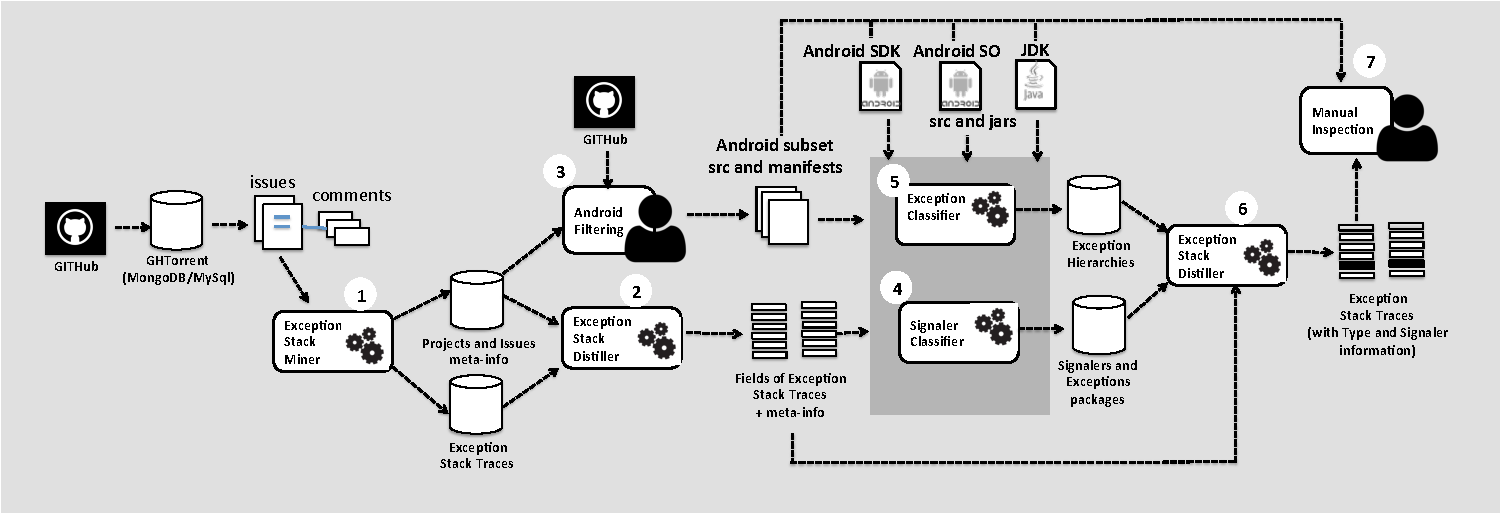
\includegraphics[width=\hsize]{overview.pdf}
%\caption{Overview of the study based on mixed approaches.}
%\label{fig:overviewfig}
%\end{figure*}



\subsection{Replication Package}
All the data used in this study will be publicly available at http://.....
Specifically we provide: (i) all issues related to Android projects found
in GITHub and Google Code used in this study; (iii) all stack traces extracted
from issues (ii) the results of manual inspection steps; (iv) the tool developed 
in this work to support stack trace extraction and distilling.

Next section presents the results for each of the study phases, providing both a
quantitative and qualitative analysis of the outcomes.

\section{The Study Results}
\label{sec:result}

%To answer this question, we mined from every extracted stack trace the top level
%exception being signaled, its signaler (the first method signature frame after
%the exception), the root exception (the exception which initiated the stack
%trace, defined on the bottom of the stack), and the root signaler. The
%intermediate elements that compose a stack trace as shown in
%Figure~\ref{fig:wrapping} (i.e., the intermediate causes and its execution
%stacks) were not be considered in the analysis.
%~\todo{Move this to the previous section? IMO, It is better to keep all facts
%about how we did the research in one place
%RSC: I WAS ABOUT TO MOOVE BUT THERE WAS ALREADY A SIMILAR TEXT ON 
%THE EXCEPTION DISTEILLER}

This section presents the results aimed at answering the research 
questions presented before.

\subsection{What can the Common Root Exceptions tell us? }

After distilling the information available on the exception stack traces we could find 
the the exceptions commonly reported as the root causes of stack traces.
Table \ref{tab:topten} illustrates the top 10 root causes found in the study,
 ranked by the number of distinct project repositories on which they were reported. 
The table shows: the number of times each exception was reported as 
the root cause of a stack trace, the number of distinct projects reporting such causes on stack traces, 
and the percentages of such in relation to all reported exceptions and analyzed projects respectively.
It also presents the whether the method responsible for signaling the exceptions were
part of Android, the application itself, libcore, or a third-party library as presented in Table  \ref{tab:signalers} 

% \footnote{Nine exception stack traces contained only elements of JVM and were discarded from the analysis}.

%For each exception we could discover the number of times it was reported as the root caused on exception stack traces,
%the number of distinct projects on which such stacks were defined (and consequently its
%popularity) and the of times it was signaled by different signaler types. We
%could calculate the popularity of each root cause, considering the number of
%distinct projects they were found and the whole set of projects analyzed with at
%least one stack trace (482). Table~\ref{tab:topten} 
%and Figure~\ref{fig:androidsignaler} presents the mined data.


%SELECTS:
%SELECT COUNT(distinct(repo)) FROM STACKTRACESUMMARY WHERE MAIN_CAUSE LIKE '%java.lang.NullPointerException%'
%and repo !='android';


%SELECT COUNT(*) FROM STACKTRACESUMMARY WHERE MAIN_CAUSE LIKE '%java.lang.IllegalStateException%'
%and repo !='android' AND MAINSIGNALER_FROM LIKE '%ANDROID%';



%java.lang.NullPointerException            & 254 /  78  & 52,70\%  & 1225 / 439  & 30,08\% & 473 /  26  & 18 /  & 595 / 241 & 137 / 169 \\  %LIBORAPP=408
%java.lang.IllegalStateException          & 99 / 21  & 20,54\%  & 234 / 44  & 5,75\%  & 165 / 15 & 12  / 0 & 36  / 5 & 20 / 24  \\
%java.lang.IllegalArgumentException          & 94 / 48  & 19,50\% & 255 / 98  & 6,26\% & 146 / 41 & 6 / 0 & 64 / 31  & 39  / 26  \\
%java.lang.RuntimeException                & 91 / 31 & 18,88\% & 232 / 87  & 5,70\%  & 167 / 33 & 1 / 0 & 47 / 17 & 17 / 37   \\
%java.lang.OutOfMemoryError                 & 56  / 22  & 11,62\% & 180 / 57 & 4,42\% & 121 / 18 & 15 / 0 & 17 / 18  & 23 / 13  \\
%java.lang.NoClassDefFoundError           & 52  / 15 & 10,79\%  & 73 / 21   & 1,79\%  & 9 / 1   & 0 / 0  & 37 / 9  & 26 / 11   \\
%java.lang.ClassCastException             & 49  / 15 & 10,17\%  & 94 / 36   & 2,31\%  & 43 / 3  & 0  / 0 & 40 / 15  & 11 / 18  \\
%java.lang.IndexOutOfBoundsException       & 47  / 15 & 9,75\%   & 127 / 39  & 3,12\% & 47 / 2  & 0/0  & 71/22  & 8 / 14    \\
%java.lang.NoSuchMethodError               & 40 / 14  & 8,30\%  & 57 / 23  & 1,40\%  & 9  /  0  & 0  / 0 & 39 /  17    & 9 / 6  \\
%java.util.ConcurrentModificationException & 38 / 5 & 7,88\% & 54 / 11  & 1,33\%   & 5  / 0  & 0  / 0 & 43 / 3 & 6 / 7  \\

%java.lang.IllegalStateException          & 99 / 21  & 20,54\%  & 234 / 44  & 5,75\%  & 165 / 15 & 12  / 0 & 36  / 5 & 20 / 24  \\
%java.lang.IllegalArgumentException          & 94 / 48  & 19,50\% & 255 / 98  & 6,26\% & 146 / 41 & 6 / 0 & 64 / 31  & 39  / 26  \\
%java.lang.RuntimeException                & 91 / 31 & 18,88\% & 232 / 87  & 5,70\%  & 167 / 33 & 1 / 0 & 47 / 17 & 17 / 37   \\
%java.lang.OutOfMemoryError                 & 56  / 22  & 11,62\% & 180 / 57 & 4,42\% & 121 / 18 & 15 / 0 & 17 / 18  & 23 / 13  \\
%java.lang.NoClassDefFoundError           & 52  / 15 & 10,79\%  & 73 / 21   & 1,79\%  & 9 / 1   & 0 / 0  & 37 / 9  & 26 / 11   \\
%java.lang.ClassCastException             & 49  / 15 & 10,17\%  & 94 / 36   & 2,31\%  & 43 / 3  & 0  / 0 & 40 / 15  & 11 / 18  \\
%java.lang.IndexOutOfBoundsException       & 47  / 15 & 9,75\%   & 127 / 39  & 3,12\% & 47 / 2  & 0/0  & 71/22  & 8 / 14    \\
%java.lang.NoSuchMethodError               & 40 / 14  & 8,30\%  & 57 / 23  & 1,40\%  & 9  /  0  & 0  / 0 & 39 /  17    & 9 / 6  \\
%java.util.ConcurrentModificationException & 38 / 5 & 7,88\% & 54 / 11  & 1,33\%   & 5  / 0  & 0  / 0 & 43 / 3 & 6 / 7  \\
%
%java.lang.NullPointerException	&	254	/	78	&	52,70\%	&	1225	/	439	&	30,08\%	&	473	/	52	&	18	/	2	&	595	/	241	&	137	/	143	\\	%LIBORAPP=408
%java.lang.IllegalStateException	&	99	/	21	&	20,54\%	&	234	/	44	&	5,75\%	&	165	/	20	&	12	/	19	&	36	/	5	&	20	/	19		\\
%java.lang.IllegalArgumentException	&	94	/	48	&	19,50\%	&	255	/	98	&	6,26\%	&	146	/	49	&	6	/	6	&	64	/	31	&	18	/	26		\\
%java.lang.RuntimeException	&	91	/	31	&	18,88\%	&	232	/	87	&	5,70\%	&	167	/	36	&	1	/	1	&	47	/	17	&	17	/	34		\\
%java.lang.OutOfMemoryError	&	56	/	22	&	11,62\%	&	180	/	57	&	4,42\%	&	121	/	20	&	15	/	1	&	17	/	18	&	23	/	11		\\
%java.lang.NoClassDefFoundError	&	52	/	15	&	10,79\%	&	73	/	21	&	1,79\%	&	9	/	1	&	0	/	0	&	37	/	9	&	26	/	11		\\
%java.lang.ClassCastException	&	49	/	15	&	10,17\%	&	94	/	36	&	2,31\%	&	43	/	12	&	0	/	0	&	40	/	15	&	11	/	9		\\
%java.lang.IndexOutOfBoundsException	&	47	/	15	&	9,75\%	&	127	/	39	&	3,12\%	&	47	/	6	&	0		0	&	71	/	22	&	8	/	10		\\
%java.lang.NoSuchMethodError	&	40	/	14	&	8,30\%	&	57	/	23	&	1,40\%	&	9	/	1	&	0	/	0	&	39	/	17	&	9	/	5		\\
%java.util.ConcurrentModificationException	&	38	/	5	&	7,88\%	&	54	/	11	&	1,33\%	&	5	/	0	&	0	/	0	&	43	/	3	&	6	/	7		



\begin{table*}
  \centering
  \begin{tabular}{rcccccccc}
    \hline
    \bfseries{Root Exception} &  \multicolumn{2}{c}{\bfseries{Projects (GH\&CG)}} &  \multicolumn{2}{c}{\bfseries{Occurrences (GH\&CG)}} & \textsf{Android} & \textsf{Libcore} & \textsf{App} & \textsf{Lib} \\
    & \bfseries{\#} &  \bfseries{\%} & \bfseries{\# } & \bfseries{\% } &&&&\\
    \hline

java.lang.NullPointerException	&	332	&	51,96\%	&	1664	&	27,71\%	&	525	&	20	&	836	&	280	\\
java.lang.IllegalStateException	&	120	&	18,78\%	&	278	&	4,63\%	&	185	&	31	&	41	&	39	\\
java.lang.IllegalArgumentException	&	142	&	22,22\%	&	353	&	5,88\%	&	195	&	12	&	95	&	44	\\
java.lang.RuntimeException	&	122	&	19,09\%	&	319	&	5,31\%	&	203	&	2	&	64	&	51	\\
java.lang.OutOfMemoryError	&	78	&	12,21\%	&	237	&	3,95\%	&	141	&	16	&	35	&	34	\\
java.lang.NoClassDefFoundError	&	67	&	10,49\%	&	94	&	1,57\%	&	10	&	0	&	46	&	37	\\
java.lang.ClassCastException	&	64	&	10,02\%	&	130	&	2,16\%	&	55	&	0	&	55	&	20	\\
java.lang.IndexOutOfBoundsException	&	62	&	9,70\%	&	166	&	2,76\%	&	53	&	0	&	93	&	18	\\
java.lang.NoSuchMethodError	&	54	&	8,45\%	&	80	&	1,33\%	&	10	&	0	&	56	&	14	\\
java.util.ConcurrentModificationException	&	43	&	6,73\%	&	65	&	1,08\%	&	5	&	0	&	46	&	13	\\
\\

    \hline
  \end{tabular}
\caption{Root Exceptions occurrences and popularity in repositories hosted in Google Code (GC) and GitHub(GH).}
\label{tab:topten}
\end{table*}

%\begin{figure}
%\centering
%\includegraphics[width=\hsize]{top_exceptios_android_new2.pdf}
%\includegraphics[width=\hsize]{top_exceptions_android_new}
%\caption{Top exceptions in Android repositories.}
%\label{fig:androidsignaler}
%\end{figure}
 

We can observe that most of this set is composed by exceptions defined by java.lang,
which are mostly not explicitly thrown by the developer but include
the exceptions implicitly thrown by the JVM due to programming errors 
(e.g., out-of-bounds array index, division-by-zero, access to a null reference)
 or resource limitation (e.g., OutOfMemoryError).
For such exceptions, which represent programming bugs or resource limitations, 
there is usually no proper handling besides presenting an error message to
 the user and restarting the application. Only high fault tolerant systems need to 
provide solutions to handle them. Hence, the best strategy to deal with them
is try to prevent them.

\emph{\textbf{The high number of NullPointerExceptions.}}
From this set the java.lang.NullPointerException was the most reported root cause; 27,71\% 
of the analyzed exception stack traces reported a java.lang.NullPointerException the root cause. 
Considering the frequencly of NullPointerException across projects, we could observe that
 51,96\% of all projects reported at least one exception stack trace on which the NullPoiterException
was the root cause.
 The NullPointerExceptions are mainly signaled inside the applicaiton code and the Android platform,
 although we also find NullPointerExceptions being signaled from third-party libraries. Regarding
reusable code, there is no consensus whether it is a good or bad practice to 
re-throw a NullPointerException. Some prefer to encapsulate such an exception on
IllegalArgumentException, while others~\cite{bloch2008effective} argue that the
NullPointerException makes the cause of the problem explicit and hence 
should not be wrapped.

The high prevalence of NullPointerExceptions is aligned with the findings of other 
works~\cite{kim2013predicting,fraser20131600,csallner2004jcrasher}. For instance, Sunghun et
al.~\cite{kim2013predicting} showed that in Eclipse bug report system 38\% the bugs 
related to exception handling were caused by NullPointerException; other works on robustness 
testing~\cite{maji2012empirical,csallner2004jcrasher} showed that most of the automatically 
detected bugs were due to NullPointerExceptions 
and exceptions implicitly-signaled by Java environment due to programming mistakes or resource limitations
 (as the ones found in this study).In Section ~\ref{sec:disc}  we provide further 
discussion on the NullPointerException problem, pointing 
to ways of how to mitigate it.

%\emph{\textbf{Direct instances of RuntimeExceptions being thrown.}}
%From Table ~\ref{tab:topten} we can observe that direct instances
%java.lang.RuntimeException were reported as the root cause of stacks in 19,09\% 
%of the projects, and most of such exceptions  were  thrown by the Android platform (167 out of 232).
%Throwing general exceptions, such as direct instances of RuntimeException, violates best
%practice III. It is considered a bad practice because exception type does not carry enough
%information to identify the cause of the exceptional behavior, and as a consequence developers need to relying on
%the exception message which can be neither complete nor precise~\cite{gosling2000java}.

\emph{\textbf{Classifying the Most Reported Root Exceptions.}} To get a broader view of the root causes of stack traces,
 we performed an empirical evaluation whose goal was to identify the concerns related to the most reported root exceptions. 

Since it is infeasible to inspect the code responsible for throwning every exception reported in this study.
This identification performed in this study was based on meaning that the name of the exception holds, 
its description (i.e., Javadoc documentaion), and the Java specification. To exemplify, an instance of ArrayOutOfBoundException
 usually refers to a programming mistake. Moreover, the Java specification list all exceptions related to backwardcompatibility 
issues ~\cite{javaback} (e.g., InstantiationError, VerifyError, IllegalAccessError).

Some concerns are known as sources of faults in mobile development are: concurrency ~\cite{ama2012} backward compatibility  
~\cite{McDon13}, security  ~\cite{enck2011study,was2010} and resource management (IO, Memory, Batery) ~\cite{Zhang12}.

%Moreover, the programming errors are also as a source of faults, as illustrated on the previous section.

However, there are exceptions that cannot be directly mapped to one of such concerns. Either because they are
related to programming mistakes - as illustrated on the previously. Or because they are too general (i.e.,  java.lang.Exception,
java.lang.RuntimeException, java.lang.Error). Or also because they are related to other concerns (e.g., specific to a given library).

%The list of categories is illustrated in Table~\ref{tab:categories}. 

To perform such mapping, we selected a subset of all reported root exceptions. This subset was composed by 100 root exceptions 
which were reported on 95\% of all stack traces analyzed in this study.

Hence, based on the inspection of the source code and Javadoc related to each exception,  and Java specification, we identified the concern
releated to each root exception. Than we could calculate the prevalence of a concern on the reported stack traces using the following metric.
Given that: Stacks is the complete set of stacks found in this study, Lc is the list of root causes related to a given concern (as identified on the study),
 and Stacks[Lc] the list of issues that mentions the concern. The prevalence of a concern could be given by the formula: Stacks[Lc]/Stacks.

Table~\ref{tab:tophundrend} illustrates the result of such mapping.

 
% When the root exceptions that were too general, or related to other concerns 
% were also maped to these additional categories. Table~\ref{tab:tophundrend} illustrates the result of such mapping.%
%\begin{table}
%  \centering
%  \begin{tabular}{|p{2cm}| p{5cm}|}
%    \hline
%    \bfseries{Category} & \bfseries{Description} \\
%    \hline
%      Programming logic &  Exceptions thrown by the JVM when the 
% evaluation of an expression violates the normal semantics of language (e.g., 
% out-of-bounds array index, division-by-zero, access to a null reference). \\ \hline
%      Resources (IO, Memory, Batery)  & Exception releated to the manipulation or restriction of resources (e.g., file, network, memory) \\ \hline
%      Security                               & Exception releated to security issues (e.g. password validation, criptography) \\ \hline
%      Concurrency                            & Exceptions related to multi-threaded programming \\ \hline
%      Backward compatibility                 &  A list of exceptions related to backward compatibility - a complete list can be found here [ref]  \\ \hline
%      Specific Exceptions              & Exceptions created for specific applications, frameworks or libraries \\ \hline
%      General (Exception, Error, Runtime)    & The top level exceptions in Java    \\ \hline
%    \hline
%  \end{tabular}
%  \caption{Description of categories.}
%  \label{tab:categories}
% \end{table}



\begin{table}
  \centering
  \begin{tabular}{lrr}
    \hline
    \bfseries{Category} &  \bfseries{\% Occurrences on stacks} \\
    \hline
      Programming logic (java.lang and util) &  52,0\%\\ 
      Resources (IO, Memory, Batery)       &   23,9\% \\ 
      Security                               &  4,1\%\\  
      Concurrency                            &  2,9\% \\ 
      Backward compatibility                 & 5,5\% \\ 
      Specific Exceptions               &  4,9\%\\ 
      General (Error, Exception, Runtime)    &  6,7\%\\
  \end{tabular}
  \caption{Identifying the concerns related to root exceptions}
  \label{tab:tophundrend}
\end{table}

To ensure the quality of the process, three independent coders classified a randomly selected
sample of 25 exception types (from the total 100) using the same list of concerns;
the interater agreement was high (96\%). We could also observe that
We can therefore assume that the categories are descriptive 
enough for covering the range of exception types analyzed.

These study showed that the programming mistakes associated to the most reported root causes. 
However, they may be interactly related to one of the other concerns. For  instance, a concurrency problem may 
lead to a NullPointerException. 

\noindent \fbox{ \begin{minipage}{0.96\columnwidth} \emph{
A multitude of programming mistakes were reported as the main causes of exception stack traces.
51,96\% of all projects reported at least one exception stack trace on which the NullPoiterException
was the root cause.
}
\end{minipage}}



%TODO: Discuss about the interater agreement here...
%\subsection{Sizes of Stack traces}
%Concerning the size of the stacks (i.e. the number of frames composing them), we
%could observe that  sometimes it exceeded 100 frames (158 stack frames).
%Manually inspecting the corresponding execution trace was caused by one of the
%two reasons: recursive calls or exceptions signaled by a method defined deep
%down in a reused framework; exceptions successively wrapped. Irrespective of the
%reason, in exception flows involving many methods, it is practically impossible
%to handle an exception in a way other than exiting the application, as at the
%place the exception occurs there is hardly enough contextual information to
%perform recovery actions.

%Considering only the packages of each exception we could observe that 81,28\%
%of all analyzed set of stack traces reported exceptions defined by java.lang
%(see Table XXX).

%\begin{table}
% \centering
%\begin{tabular}{lrrrr}
%    \hline
% \bfseries{rank} & \bfseries{package} & \bfseries{occurr} &  \bfseries{\%occur} & % \bfseries{projects} \\
%     \hline
%1 & java.lang         & 19471 & 81,28\% & 3080 \\
%2 & java.io           & 1222  & 5,10\%  & 509 \\
%3 & java.net          & 740   & 3,09\%  & 311 \\
%4 & java.util         & 689   & 2,88\%  & 287 \\
%5 & java.lang.reflect & 115   & 0,48\%  & 78 \\
%\hline
%  \end{tabular}
%\caption{Top 5 most popular packages associated to the root exceptions of stack traces}
%\label{tab:toptenpopular2}
%\end{table}

%\noindent \fbox{
%\begin{minipage}{0.96\columnwidth} 
%\emph{RQ2: Most exceptions are due to programming mistakes
%or generally irrecoverable errors.}
%\end{minipage}}

\subsection{What can the Types of Root Exceptions tell us?}
%\subsection{Exploring the Information Embedded on Exception Types}
%\subsection{The Exception Types and What They can Tell us? }

Besides distilling the information available on stack traces (i.e., exception signalers, root causes, exception wrappings),
we mined the exception types (i.e., RuntimeException, checked Exception or Error) related to each exception reported on stack traces -
to do so we used the source code and byte code analyses implemented on Exception Miner. 

 Table~\ref{tab:typeroottab} presents the types of root causes of all stack traces reported on the analyzed issues. As we can see 
from Table ~\ref{tab:typeroottab},  most of the reported exceptions signaled (explicilty or implicitly by the JVM) on methods defined
 on the Android Plaform on on the application itself. 

On the other hand, most of the reported exceptions signaled by the set of 
libraries reused by Android platform were checked exceptions. Such libraries are referred in
this work as libcore and is composed by org.apache.harmony, org.w3c.dom, sun.misc, 
org.apache.http, org.json, org.xml, javax. It is pointed as a good practice
for libraries (see Section~\ref{sec:best}) because by using checked exceptions
a library can define a precise exception interface ~/cite{miller1997issues} to its clients. Such
libraries are heavily used in several projects, and such precise exception
interface may be related to the library's maturity.

%SELECT COUNT(*) FROM STACKTRACESUMMARY WHERE
% repo !='android'  AND MAIN_EXTENDS LIKE 'RUNTIME%' 


%SELECT COUNT(*) FROM STACKTRACESUMMARY WHERE
%repo !='android'  AND MAIN_EXTENDS LIKE 'RUNT%' AND MAINSIGNALER_FROM like 'APP%';

% \bfseries{Root Cause Type} & \bfseries{Android} & \bfseries{Libcore} & \bfseries{App} & \bfseries{Lib}  & \bfseries{All}\\
% Runtime	&	1075 / 260	&	56  / 17	&	1446 / 397	&	374	/  316  &	2951 / 943\\
%Error	       &	 144	 / 44              &	34 / 12	&	168	 / 134              &	105	 / 62           &	451 /  240	\\
%Checked	&	193	/ 83            &	230 / 84	&	139	  / 174          &	145 / 422	           &	624  / 734	\\
%Throwable	&	0 /0	       &	0	&	1 / 1	             &	0	     / 0               &	1 / 1	\\
%Undefined	&	1 / 3 	&	0	&	6 / 	12		&	8 / 30	   &	15 / 45	\\ %22 DISTINCT EXCEPTIONS AND 9 IN GIT

%Runtime	&	1075 / 160	&	56 	&	1446 / 397	&	374	/  386  &	2951 / 943\\
%Error	       &	 144	 / 32              &	34	&	168	 / 134               &	105	 / 74           &	451 /  240	\\
%Checked	&	110	   / 39           &	230	&	139	  / 174            &	145	 / 466           &	624  /  679	\\
%Throwable	&	0 /0	       &	0	&	1 / 1	             &	0	     / 0               &	1 / 1	\\
%Undefined	&	1 / 1 	&	0	&	6 / 	12		&	8	/ 32	   &	15 / 45	\\ %22 DISTINCT EXCEPTIONS AND 9 IN GIT
%All		& 1330	&	320	&	1760	&	632	&	4042	\\


%Runtime	&	1235	&	56 	&	1843	&	760  &	3894\\
%Error	       &	 176              &	34	&	302               &	179          &	691	\\
%Checked	&	149           &	230	&	313            &	611           &	1303	\\
%Throwable	&	0        &	0	&	2             &	0	                    &	2	\\
%Undefined	&	2 	&	0	&	18		& 40	   &	60	\\ %22 DISTINCT EXCEPTIONS AND 9 IN GIT
%  \hline
%All		& 1562	& 320	& 	2478	& 1590	& 5950 \\

%FILTRAR LIBCODE:
%FILTRO ANDROID: 74 (com.android) 122(com.google)
%SELECT REPO, main_signaler, *
%  FROM stacktracesummary where mainsignaler_from='LIB_or_APP' AND main_signaler like 'com.google%' ;

\begin{table}
\centering
\begin{tabular}{lccccc}
    \hline
    \bfseries{Root Cause Type} & \bfseries{Android} & \bfseries{Libcore} & \bfseries{App} & \bfseries{Lib}  & \bfseries{All}\\
    \hline

Runtime	&	1335	&	73	&	1843	&	690  &	3894\\
Error	       &	 188              &	 46	&	302             &	167	           &	691	\\
Checked	&	276           &	314	&	313          &	567	           &	1358	\\
Throwable	&	0	       &	0	&	2            &	0	     / 0               &	2	\\
Undefined	&	4	&	0	&	18		&	38	   &	60	\\
 \hline
All		& 1803	&	433	&	2478	&	1462	&	6005	\\
    \hline
  \end{tabular}
\caption{Types of root exceptions.}
  \label{tab:typeroottab}
\end{table}

%\begin{figure}
%\centering
%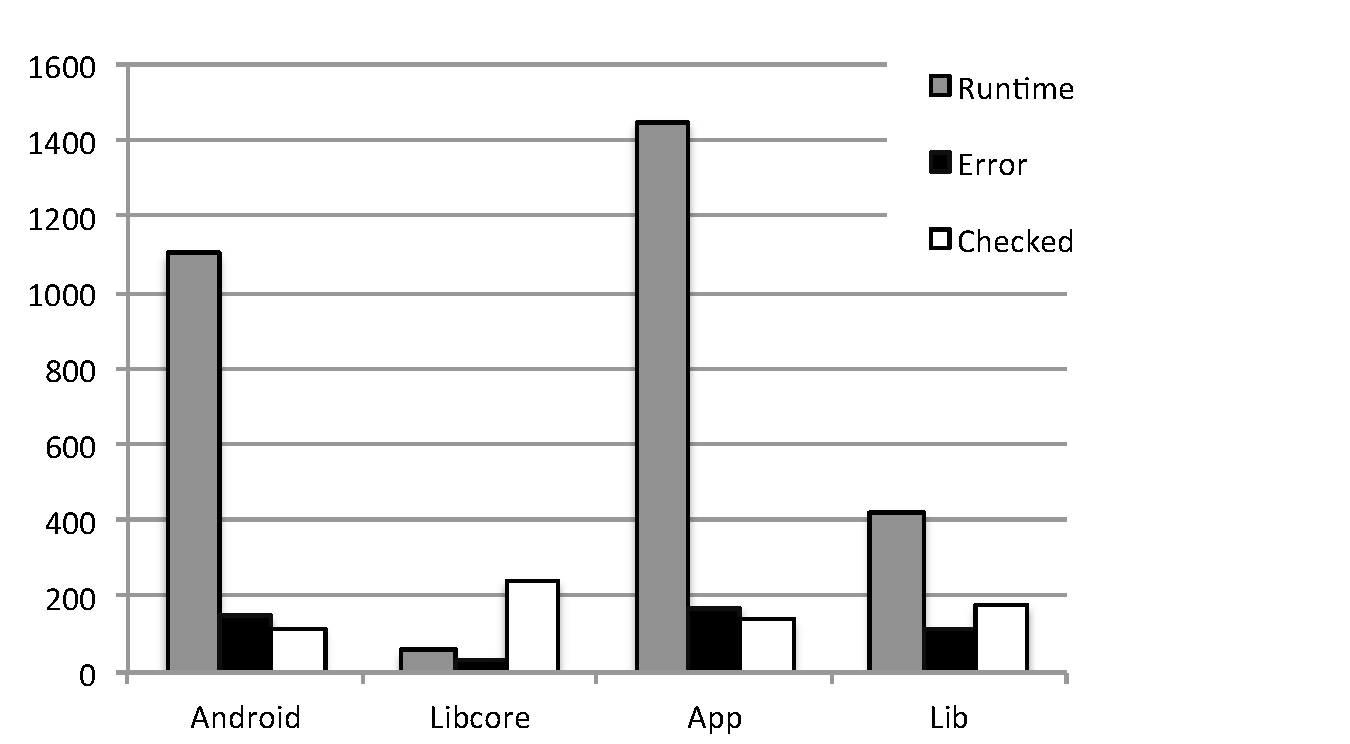
\includegraphics[width=\hsize]{chart_exceptiontypes.pdf}
%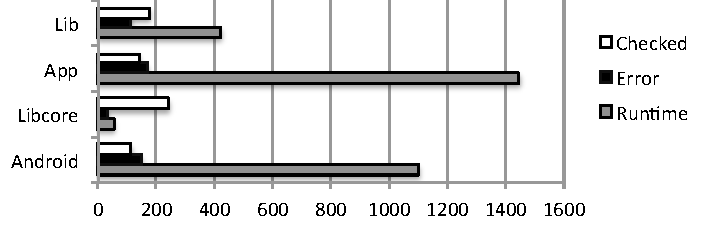
\includegraphics[width=\hsize]{exception_types.pdf}
%\caption{Distribution of Checked and Unchecked exceptions.}
%\label{fig:typeroot}
%\end{figure}

% REMOVED BECAUSE WE DO NOT HAVE SPACE TO DISCUSS IT, AND IT IS NOT WELL
% CONNECTED WITH PREVIOUS.
%\subsection{Uncaught Checked Exceptions}
%Although most of the  reported exceptions were runtime, we could also find checked
%exceptions as the root causes of stack traces reported on issues. A checked exception
%can remain uncaught in two circumstances: if all methods on the execution trace
%on which this exception flows explicitly specifies the exception, or if the
%checked exception is wrapped in a runtime and than re-thrown. Since checked exceptions 
%should be used to represent recoverable conditions, ignoring a
%checked exception, is considered a bad practice. As mentioned before, when the developer is confronted
%with a checked exception, the designer of the API is telling him to handle the
%exceptional condition. To better understand what was causing checked exceptions
%to scape from being handled we investigated the kinds of wrappings that happened
%on stacks the stacks.  Next sections presents the wrappings found and discuss
%about them.

\emph{\textbf{Undocumented Runtime Exceptions}}.
However, we can also observe a considetable amount of 
runtime exception signaled on library reused by apps.
In order to evaluate if  best practice IV was being obeyed, we inspected the   
signature of each method signaling a runtime exception. 
We inspected methods of the Android Plaftorm and 
the libraries, because both are  third  party code reused 
by the Android apps. In this task we filtered out all the exceptions implicitly 
signaled by  JVM (due to programming mistakes) 
since these exceptions should not be documented on the 
method signature. 

As a result of this inspection, we could observe that only 1 method out of 118 inspected signalers
 (i.e., 0,8\%) documented the explicitly thrown runtime exception in a Javadoc comment; and none of these methods
included the runtime exception  (reported on the stack) as part of the exception interface of the method (i.e., using 
throws clause on method signature). This result is aligned with the results of other study conducted by from 
Sacramento et al ~\cite{sacramento2006unchecked} which observed that the
runtime exceptions in .Net programs are most often not documented.

Such undocumented runtime exceptions represent a threat to system robustness, specially
when such exceptions are thrown then the third party code is invoked inside the application 
(e.g. libraries, or framework utility code). In such cases the client usually do not have access to 
the source code, and in the absence of
the exception documentation it is very difficult or even impossible for the client of such third party code to 
protect the application against undocumented runtime exceptions. As a consequence, the
 undocumented runtime exception may remain uncaught and lead to system crashes.



%SELECT repo, *
% FROM stacktracesummary where stack like '%getDeclaredMethods%';


\noindent \fbox{ \begin{minipage}{0.96\columnwidth} \emph{
 Only 0,8\% of the methods documented the explicitly signaled runtime exceptions. 
}
\end{minipage}}

\subsection{What can the Exception Wrappings tell us?}
%\subsection{Exploring the Information Embedded on Exception Wrappings}

Table~\ref{tab:wrappingandroid} presents the wrappings found in this study for all
stack traces found in Android repositories. As we can see, some of the checked
exceptions were indeed wrapped in runtime exceptions or even errors.


%SELECT COUNT(*) FROM STACKTRACESUMMARY WHERE
%repo !='android'  AND ROOT_EXTENDS LIKE 'CHECKED%' AND EXCEPTION_EXTENDS LIKE 'RUNTIME' 

%SELECT COUNT(*) FROM STACKTRACESUMMARY WHERE
%repo !='android'  AND ROOT_EXTENDS LIKE 'CHEC%' AND EXCEPTION_EXTENDS LIKE 'RUN%'; 

%SELECT COUNT(*) FROM STACKTRACESUMMARY WHERE
%repo !='android'  AND ROOT_EXTENDS LIKE 'CHEC%' AND EXCEPTION_EXTENDS LIKE 'RUN%'
%and SIGNALER_FROM LIKE 'LIB%'; 

 %Runtime &  Checked   & 70  / 18 & 114 /  34 &  66 /  9  &  0 /  & 19 / 19 &  29 / 6 \\
      %Runtime   &  Error   & 38  \ 8  & 57    &  50 \ 8  &  0   & 6 \ 2  &  1   /  0\\
%      Checked &  Runtime   & 12 \ 5  & 22 \ 9 & 4 &  0  & 9 \7 &  9 \ 2 \\
%      Checked & Error      & 7 \ 1 &  8 & 5  &  0  & 0 \ 1 &  3 \0 \\
 %     Error & Checked      & 4 \ 10  &  7 & 0  \ 6  &  7  & 0 \6 &  0   \ 8    \\
%      Error & Runtime     & 6 \ 2  &  13   & 1 &  1  & 0 \ 1 &  11 \ 3    \\

\begin{table*}
  \centering
  \begin{tabular}{llcccccc}
    \hline
    \bfseries{Wrapper Type}  &  \bfseries{Root Cause Type} &  \bfseries{Projects}  &  \bfseries{Occurrences} & \textsf{Android} & \textsf{Java/Libcore} & \textsf{Lib} & \textsf{App}  \\
    \hline
      
      Runtime &  Checked   & 88 & 148 &  75  &  0   & 38 &  35 \\
      Runtime   &  Error   & 46  &  67    &  58  &  0   & 8  &  1   \\      
      Checked &  Runtime   & 17  & 31 & 4 &  0  & 16 &  11 \\
      Checked & Error      & 8 &  9  & 5  &  0  &  1 &  3  \\
      Error & Checked      & 14 &  27 &  6  &  7  &  6 &   8    \\
      Error & Runtime     & 8  &  17   & 1 &  1  & 1 &  14    \\

  \hline
      %none   & Runtime   &  2360 & 359 \\
      %none  &   Checked  & 422  & 117 \\
      %none  &   Error   & 381  & 141 \\
      %none &  Undefined  &  15   & 10  \\
      %none & Throwable  &  1    & 1 \\
     %\hline
      %Runtime   & Runtime & 560  & 182 \\    
      %Checked   & Checked & 98   & 42  \\
      %Error     & Error   & 15   & 14  \\
    %\hline
  \end{tabular}
\caption{Wrappings comprising different exception types.}
\label{tab:wrappingandroid}
\end{table*}



This analysis revealed unexpected wrappings such as: Error wrapping a Checked 
exception; a Runtime wrapping and Error; and an Error wrapping a Runtime.
Java is the only language that provides a hybrid exception model 
which offers  different types to represent different exception behaviors (i.e., error, 
runtime and checked) (see Section~\ref{sec:best}). For instance,
according to Java specification, Errors should not be handled inside the system 
since they usually represent unrecoverable conditions
detected by the JVM (e.g.,  OutOfMemoryError). On the other hand, checked exceptions should
represent recoverable conditions. Next we discuss and exemplify the cross-type wrappings
 found in this study.

\emph{\textbf{Runtime wrapping Checked Exception.}} Such wrapping was 
detected on 88 projects. Inspecting the 
elements responsible for performing such wrapping, we could observe that
approximately  50\% of such wrappings were performed on methods defined on Android
Platform. 

Taking a closer look on the methods responsible for such wrappings,
 we could observe that approximately 41\% of them were performed by a single class,
 named ActivityThreat. 

This class is responsible for managing the life cycle of  Android Activities - 
invoking the life cycle methods (i.e. onCreate(), onPause()) for every Activity 
(window) of an Android app.
Figure ~\ref{fig:snippets} (a) presents a code snippet of one the methods of 
ActivityThrea,  the one responsible for invoking the Activitiy's onCreate method. 
As we can see from lines 4-8,
 in case any exception is thrown in the context of such try-catch block, 
it is wrapped in a general Runtime exception and re-thrown.

\begin{table}
\centering
\begin{tabular}{lll}
    \hline
 \bfseries{Signaler class} &  \bfseries{Wrapper Type} & \bfseries{Ocurrences} \\
    \hline
android.app.ActivityThread & java.lang.RuntimeException & 61\\
android.view.LayoutInflater & android.view.InflateException &  7 \\
android.os.AsyncTask & java.lang.RuntimeException &  7\\
\hline
  \end{tabular}
\caption{Top 3 Runtime-Cheked wrappers.}
\label{tab:wrapping01}
\end{table}

%MOVED TO THE PICTURE
%{\footnotesize
%\begin{verbatim}
%1. private Activity performLaunchActivity(...) {
%2.  try {
%3.   ...
%4.   ...callActivityOnCreate(...);
%5.  } catch (Exception e) {
%6.    ...
%7.   throw new RuntimeException(..., e);
%8.  }
%9.}
%\end{verbatim}
%}

%SELECT SIGNALER_method, COUNT(*) AS N
%  FROM stacktracesummary WHERE ROOT_EXTENDS='CHECKED' AND EXCEPTION_EXTENDS='RUNTIME' and
%  ( SIGNALER_method like '%onDestroy%' or
%   SIGNALER_method like '%onCreate%' or
% SIGNALER_method like '%onStart%' or
% SIGNALER_method like '%onResume%' or
% SIGNALER_method like '%onPause%' or
% SIGNALER_method like '%onStop%' or
% SIGNALER_method like '%onDestroy%' )
%   GROUP BY SIGNALER_method
%  ORDER BY N DESC;

%SELECT COUNT(*) AS N
 % FROM stacktracesummary WHERE ROOT_EXTENDS='CHECKED' AND EXCEPTION_EXTENDS='RUNTIME' and
 % ( stack like '%onDestroy%' or
 %  stack like '%onCreate%' or
% stack like '%onStart%' or
% stack like '%onResume%' or
% stack like '%onPause%' or
% stack like '%onStop%' or
% stack like '%onDestroy%' );

%GC = 6

%However, since the Activity life clycle method (i.e., callActivityOnCreate(...)) that is invoked in this block,
% do not include checked exceptions on its signatures. Hence they could not throw a checked exception to be handled 
%in the method illustrated above. However the code inspection performed on such wrappings revelaed an
%``undocumented checked exception" signaled by this life cycle method.

%\emph{\textbf{Undocumented Checked Exceptions.}} There are usually
%2 possible for a checked exception to be thrown by a method:
%it can either be specified on the method signature or it can be wrapped in a 
%runtime exception and re-thrown. 

Inspectioning the source code, of the methods involved in this kind of wrapping,
revealed another fragility: a checked exception thrown by a native method and not
declared on the exception interface of thes methods signaling them. Such native method 
was defined on Android Platform -  which uses Java Native Invocation (JNI) to access 
native C/C++ code. 

The code snippet in Figure ~\ref{fig:snippets} (d) illustrates this fragility.
 The java/lang/Class declares a native method named getDeclaredMethods. 
The Java-side declaration of of this method does not have any throws clause, 
leading programmers and the compiler to think that no checked exceptions can be thrown.
 However, the C-code implementation did throw a "checked exception" NoSuchMethodException, 
violating the declaration. The Java compiler, could not detect this violation because it does 
not perform static exception checking on native methods. This type of bug is hard to diagnose
because the developer usualy do not have access to the native implementations. 
Consequently, since it is not expected by the programmer, when such method throws 
this exception, such undocumented exception may remain
uncaught and cause the app to crash, or may be mistakenly handled by subsumption - 
The exception stack traces reporting this scenario is actually a real bug of Android 
Gingerbread version (which still accounts for 13.6\% of devices running Android).

Among the Android projects on which this exception stack trace was reported we can cite:
PageTurner (206 stars, 130 forks, 1184 commits), ActionBarSherlock (6,041 stars, 
3,436 forks, and 1479 commints), otto (1,618 stars,	342 forks, 	177 commints).

% Several types of exceptions were  wrapped the RuntimeExceptions thrown by the 
% ActivityThread. Table X illustrates them.
% #\begin{table}
% \centering
% \begin{tabular}{lll}
%    \hline
%    \bfseries{wrapper} & \bfseries{root} & \bfseries{\#} \\
%    \hline
% java.lang.RuntimeException & java.lang.ClassNotFoundException &	32 \\
% java.lang.RuntimeException & java.lang.NoSuchMethodException &	6 \\
% java.lang.RuntimeException & java.lang.InstantiationException) & 5 \\
% ...andlyticsproject.NetworkException & org.apache...HttpResponseException &	5\\
% android.view.InflateException & java.lang.NoSuchMethodException & 4 \\
% \hline
%  \end{tabular}
% \caption{Elements responsible for the wrapping.}
% \label{tab:wrapping01}
% \end{table}


% \begin{table}
% \centering
% \begin{tabular}{lll}
%   \hline
%   \bfseries{Exception} & \bfseries{Ocurrences} \\
%   \hline
% java.lang.RuntimeException &	69 & 61\% \\
% android.view.InflateException	& 10 & 8,7\% \\
% com.github.andlyticsproject.console.NetworkException	& 7 & - \\
% java.lang.IllegalStateException	& 6 & - \\
% \hline
%  \end{tabular}
% \caption{Elements tresponsible for the wrapping.}
% \label{tab:wrapping01}
% \end{table}


\emph{\textbf{Runtime Exception wrapping Error.}} We could find  64 exception stack traces 
on 46 projects on which an Error was wrapped in a runtime exception.
Manually inspecting each exception stack trace, we could observe that 44% of the wrappings were performed 
by android.os.AsyncTask. This class is responsible for dealing with asynchronous tasks in Android.
The code snippet is illustrated in Figure ~ref{wrappings} (c) shows that any throwable signaled in the context of an asynchronous 
task is converted in to a runtime and re-thrown. Some of the Erros wrapped on instances of runtime exceptions were 
java.lang.OutOfMemoryError (30), java.lang.NoClassDefFoundError (6), 
java.lang.UnsatisfiedLinkError (5), java.lang.StackOverflowErro (4), as illustrated in Table ~\ref{tab:exampeswrap}.

%ASSNCTASKS NON ANNOTATED METHODS…….
%SOME HAVE EXCEPTION INTERFACE 
%EXCEPTIONS ON MEHTODS SIGNATURE OTHERS NOT
%INCONSISTENCY…. DEPENDS ON DEVELOPERS 
%WORK INSTEAD OF TOOLS.


%{\footnotesize
%\begin{verbatim}
%protected void done() {
% ...
 %  try {
 %     ...
  % } catch (InterruptedException e) {
  %    android.util.Log.w(..., e);
  % } catch (ExecutionException e) {
  %    throw new RuntimeException("...",e.getCause());
  % } catch (CancellationException e) {
  %    ...
 %  } catch (Throwable t) {
 %    throw new RuntimeException("...", t);
 %  }
 %   ...
% }
%}
%\end{verbatim}
%}

\begin{table}
\centering

 %\begin{tabular}{|p{7.9cm} p{0.1cm}|}
\begin{tabular}{ll}
    \hline
 id & \bfseries{Runtime-Error Wrapping Examples}    \\  %\bfseries{\#}
    \hline
1 & java.lang.RuntimeException - java.lang.OutOfMemoryError  \\ %30
2 &java.lang.RuntimeException - java.lang.NoClassDefFoundError \\ %6
3 &java.lang.RuntimeException - java.lang.UnsatisfiedLinkError)  \\ %5
4& java.lang.RuntimeException -  java.lang.StackOverflowError)   \\ %4
\hline
 & \bfseries{Checked-Runtime Wrapping Examples}   \\
 \hline
5& ...android.robospice.CacheSavingException - java.lang.ClassCastException   \\ %6
6&java.lang.reflect.InvocationTargetException - java.lang.NullPointerException    \\ %3
7&java.lang.reflect.InvocationTargetException - ...ResourcesdNotFoundException  \\ %2
8&java.sql.SQLException - android.database.sqlite.SQLiteDiskIOException   \\ %2
 \hline
& \bfseries{Checked-Error Wrapping Examples}  \\
 \hline
9&java.lang.reflect.InvocationTargetException - java.lang.OutOfMemoryError  \\ %5
10&java.lang.Exception - java.lang.OutOfMemoryError   \\ %1
11&java.lang.reflect.InvocationTargetException - java.lang.NoSuchMethodError 	 \\ %1
12&java.lang.reflect.InvocationTargetException - java.lang.UnsatisfiedLinkError	 \\ %1
\hline
& \bfseries{Error-Checked Wrapping Examples}  \\
 \hline
13&java.lang.NoClassDefFoundError - java.lang.ClassNotFoundException   \\ %4
14&java.lang.AssertionError - javax.crypto.ShortBufferException)   \\ %3
\hline
& \bfseries{Error-Runtime Wrapping Examples}    \\
 \hline
15&java.lang.ExceptionInInitializerError - java.lang.NullPointerException   \\ %9
16&java.lang.ExceptionInInitializerError - java.lang.IllegalArgumentException 	 \\ %2
 \hline
  \end{tabular}
\caption{Examples of Cross-type wrappings}
\label{tab:exampeswrap}
\end{table}


\emph{\textbf{Checked wrapping Runtime Exception.}} Manually inspecting the stack 
traces we could observe that most of the wrappings were performed 
by RoboSpice (an android library that supports the creation of asynchronous long running 
tasks, which has 1.682 stars and 367 forks in GitHub) and by the reflection Java library (used by Android, 
Application and library classes). Inspecting the code related to such wrappings we could observe that
the reflection library convert every exception that happens 
when invoking a reflected method into an InvoncationTargetException (this conversion is 
performed inside native code).

%\begin{table}
%\centering
%\begin{tabular}{ll}
% \bfseries{Wrapper type - Root cause type} & \bfseries{\#}\\
% \hline
%...android.robospice.CacheSavingException - java.lang.ClassCastException & 6 \\
%java.lang.reflect.InvocationTargetException - java.lang.NullPointerException &  3 \\
%java.lang.reflect.InvocationTargetException - ...ResourcesdNotFoundException & 2 \\
%java.sql.SQLException - android.database.sqlite.SQLiteDiskIOException & 2 \\
%  \end{tabular}
%\caption{Elements tresponsible for the wrapping.}
%\label{tab:wrapping01}
%\end{table}


\emph{\textbf{Checked Exception wrapping Error.}} Almost all of these wrappings
 were also caused by the reflection library 
used by Android applications. The methods responsible for the wrappings
were also native methods written in C. Table ~\ref{tab:exampleswrap} illustrates
some oth these wrappings some of them are masking an OutOfMemoryError
into a checked exception.

%\begin{table}
%\centering
%\begin{tabular}{lll}
% \bfseries{Wrapper type - Root cause type} & \bfseries{\#}\\
% \hline
%java.lang.reflect.InvocationTargetException - java.lang.OutOfMemoryError & 5 \\
%java.lang.Exception - java.lang.OutOfMemoryError & 1 \\
%java.lang.reflect.InvocationTargetException - java.lang.NoSuchMethodError &	1 \\
%java.lang.reflect.InvocationTargetException - java.lang.UnsatisfiedLinkError&	1 \\
%  \end{tabular}
%\caption{Elements tresponsible for the wrapping.}
%\label{tab:wrapcheckerr}
%\end{table}

\emph{\textbf{Error wrapping Checked Exception.}} Some of these wrappings were performed by methods defined by java.lang.Class methods such as 
at java.lang.Class.getDeclaredFields(Native Method)
at java.lang.Class.getDeclaredConstructors(Native Method), 
while others were performed by javax.crypto package. Table X illustrates
the exception types involved in such wrappings.

%\begin{table}
%\centering
%\begin{tabular}{lll}
% \bfseries{Wrapper} & \bfseries{Root} & \bfseries{\#}\\
% \hline
%java.lang.NoClassDefFoundError & java.lang.ClassNotFoundException & 4 \\
%java.lang.AssertionError & javax.crypto.ShortBufferException) & 3 \\
% \end{tabular}
%\caption{Elements tresponsible for the wrapping.}
%\label{tab:wrapping01}
%\end{table}

\emph{\textbf{Error wrapping Runtime.}} After manually inspecting the code associated to such wrappings 
we discovered that all of them were caused by static initializers. If any exception is thrown in the context of a static initializer (i.e., static block) 
it is converted into an ExceptionInitializerError on the point where the class is first used. Table ~\ref{exampleswrap} illustrates
the exception types involved in such wrappings.

%\begin{table}
%\centering
%\begin{tabular}{ll}
% \bfseries{Wrapper type - Root cause type} & \bfseries{\#} \\
% \hline
%java.lang.ExceptionInInitializerError - java.lang.NullPointerException & 9 \\
%java.lang.ExceptionInInitializerError - java.lang.IllegalArgumentException &	2 \\
% \end{tabular}
%\caption{Elements tresponsible for the wrapping.}
%\label{tab:wrapping01}
%\end{table}


\emph{\textbf{Multiple Wrappings.}} We could also observe that in 205 stacks found
 in Android repository the exception was wrapped  more then once. One interesting 
multiple-wrapping found in Android repo was the 
following: Runtime-Checked-Runtime-Checked-Runtime-Checked-Runtime.

\noindent \fbox{ \begin{minipage}{0.96\columnwidth} \emph{
Odd wrappings were detected (e.g., a checked exception wrapping an OutOfMemoryError).
The study also detected an undocumented checked exception signaled by
  a native method defined in Android.
}
\end{minipage}}


\section{Further Discussions}
\label{sec:disc}

\begin{figure*} \centering 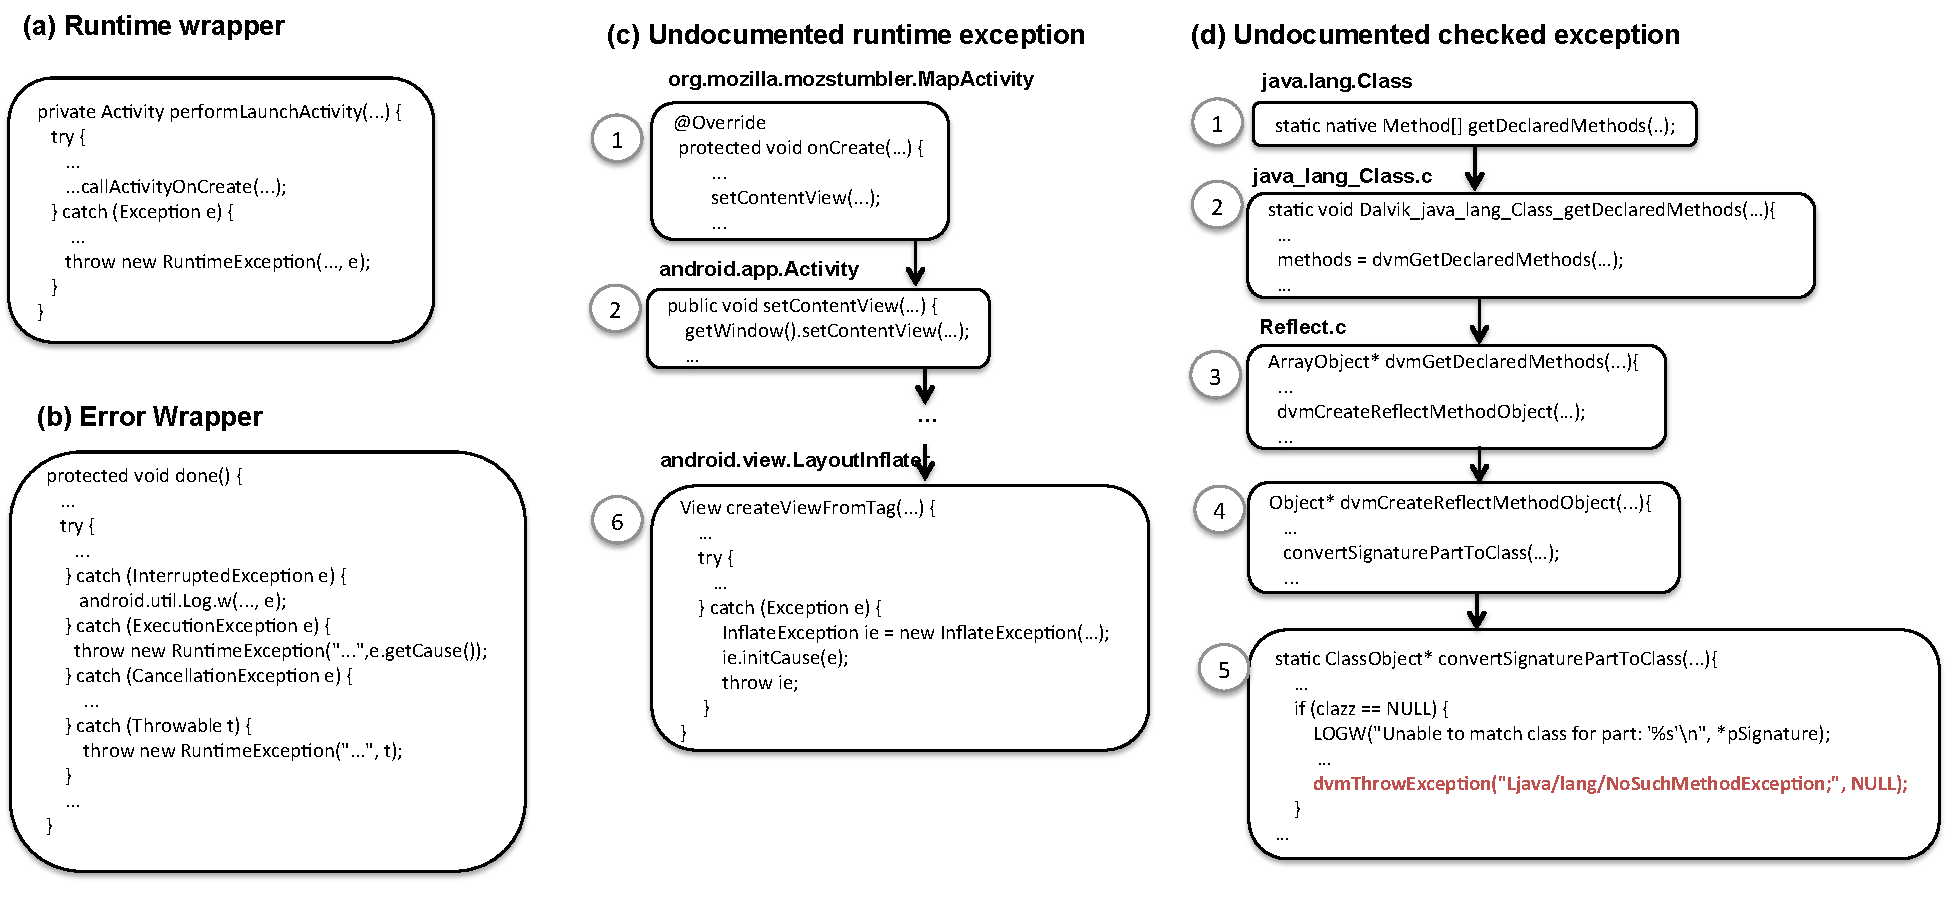
\includegraphics[scale=0.55]{codeexamples.pdf}
\caption{Code snippets illustrating fragilities on the exception-related code} \label{fig:snippets} \end{figure*}



\subsection{On the need of a rescue to the almost infeasible task of preventing uncaught exceptions}
In this study we could observe undocumented runtime exceptions thrown by third party code,
and even undocumented checked exception thrown by Java supporting library.
Such undocumented exceptions make difficult, and most of the times infeasible
for the client code to protect against `unforeseen" situations that may happen 
while calling a library code.

One may think that the solution for the uncaught exceptions 
may be to define a general handler, 
which is responsible for handling any exception that is not
adequately handled inside the applications. Although this 
solution may prevent  the system of abruptly crashing,
 such general handler will not have enough
contextual information to adequately handle the exception, 
and only tasks possible are: to present a message to the user
 and restart the application.

Such handler does not replace a carefully designed exception 
handling policy, which can hardly be designed in the absence of 
third-party documentation on the exceptions that
may the thrown by it.

On the other hand documenting runtime exceptions is a tedious and error prone task, to help developers
mitigate this problem tools should be developed to automate the documentation of runtime exceptions
scraping from library code, few solutions in this directions have been proposed so far ~\cite{van2005combining}. 

\subsection{On the cross-type wrappings as a threat to dependability}
The cross-type wrappings detected in this study points to the fact that: (1) exception 
wrappings may prevent exception types from being used according to its initial purpose
 (e.g, Errors should represent situations that should not be handled); and (2) may  be used
 to bypass the language restrictions imposed by checked exceptions  (e.g,
 checked exceptions may be wrapped in runtime exceptions).

Hence, when (mis)applied, the exception wrapping can make the exception-related code
 more complex and lead to what we call an \emph{exception handling confusion problem}.
Such problem can lead the program to
an unpredictable state in the presence of exceptions. To illustrate this problem, we can use
 one of the examples found in this study: when the developer is 
confronted with a checked exception, the designer of the API is telling him 
to handle the exceptional condition, however we could observe that in some cases the 
checked exception wrapped an OutOfMemoryError, which represent resource deficiency detected 
by the JVM which make impossible the program to recover. 

Currently there is no way of enforcing Java exception type conventions during program development.
Hence, further investigation is needed on finding ways to help developers in dealing with such
 problem, either preventing odd wrappings or enabling the developer to better deal with them or even
researches on the real usefulness of Java hybrid exception model. 


\subsection{On the null pointer problem}

Besides the explicitly thrown runtime exceptions, in this work we also observe a high number of 
stack traces reporting coding errors (out-of-bounds array index, division-by-zero, access to a null).
Such exceptions are implicitly thrown by JVM, and among them the NullPointerException 
were the reported root cause in most of the analyzed exception stack traces.

The null references was firstly introduced by Tony Hoare in ALGOL W, which after some years he called his “one-billion-dollar mistake”:

\emph{``I call it my billion-dollar mistake. It was the invention of the null reference in 1965 [...] I couldn’t resist the temptation to put 
in a null reference, simply because it was so easy to implement. This has led to innumerable errors, vulnerabilities, and system 
crashes, which have probably caused a billion dollars of pain and damage in the last forty year."}

The high number of null pointer exceptions found in this mining study shed light into a problem
that although known was not supported by large scale studies. 

This observation emphasizes the importance of solutions to avoid NullPointerExceptions, such as:
(i) lightweight intra-method null pointer analysis supported by Java8 @Nullable annotations;
(ii) inter-method null pointer analysis tools such as the one proposed by Nanda and Sinha ~\cite{nanda2009accurate};
or (iii) whether language designs which avoid null pointers, such 
as Monads ~\cite{Walde95} (i.e., used in functional languages for values that may not be available 
or computations that may fail) could improve the robustness of Java programs. 

The @Nullable annotations are used by analyzers like the Checker Framework, FindBugs, Eclipse, 
NetBeans, IntelliJ, and other commercial tools which run at compile time and detect potential null 
pointer dereferences. Android Studio 0.5.5 Released support these annotations.

%(1) mostrar a utilizacao de @nullable em projetos android. rodar em alguns e mostrar.
%Android Project Unwritten Rules (http://blog.lemberg.co.uk/android-project-unwritten-rules)
%(2) dar foco em android
%(3) falar do modelo do ciclo de vida da aplicacao e da necessidade de usar excecoes Runtime.
%(4) Local onde tratar excecao - handler padrao - politica da aplicacao. tratamento difucultado multiplas threads e assyncronos.


%\noindent\emph{Unwritten Rules of Android Exception Handling Developement}
%\noindent\emph{Dependency injection - Inversion of Control -  callback and Exceptions }  
%\subsection{Dependency injection - Inversion of Control -  callback and Exceptions}  
%\noindent\emph{How can we benefit from such cross-project crash analysis?}  


%\subsection{Inversion of Control and Exception Handling}
\subsection{On the absence of exception interface on hook methods of the Android Aplication Framework}

In this study, the analyzed stack traces involved, in one way or another, methods from the 
Android Application Framework: either framework utility methods inkoked 
by the application, or framework hook methods  (e.g., OnCreate(), onPause())  
 extended by the application and invoked by the framework (by inversion of control).
 As discussed before, some of the utility 
methods signaled ``undocumented" runtime exceptions. Additionaly, another characteristic of 
Android Platform may also be imposing obstacles to application robustness: the absence 
of exception interface (i.e., a list of exceptions that a method 
might raise during its execution) of Android rook methods.

For instance, none of the hook methods povided by the Activity class (and 
extended by every Android app) specify an exception interface. Therefore, such methods
do not stimulate the developer to think that ``something" may go wrong 
during the execution of such methods, and prepare the code to deal with them.

To make matters worse, according to Java handling model, the exception handler
 should be added on the invocation chain of the signaler.  However,  on method invocations based 
on inversion of control, the developer does not have fully access to the invocation 
chain of a method. 

Such difficulties may lead the developers into believing that by just re-throwing the exceptions they can 
forget about the exceptional situations, while focusing on the developement of the `happy path". 
This `ignore-for-now" approach may lead to the known uncaught exceptions problem~\cite{jo2004uncaught},
and unintened handler actions,  contributing to degrate apps robustness.

Rephasing Brian Foote "Everybody hates thinking about exceptions, because they’re not supposed to happen"
however one day they happen, and you need to prepare your code for it. However, further investigation
 is needed to evaluate the impact of  the absence of exception interface of Android rook methods on
app robustness.

\subsection{On the benefits of a cross-project exception stack trace analysis}  

When family of systems make use of a common core, it is possible to benefit from a cross project crash analysis like the one performed in this study.
 The not only the exception stack traces but any other bug issues reported for a group of systems can identify vulnerabilities 
that are common to more then one element of the family and are more difficult to identify in a single project analysis.
Therefore tools such as the one developed in this study may allow the developers to 
benefit from the faults happening on different systems.  

%It can be a way of dealing with the test case explosion problem related to framework test.
%Let the products test and report the crahes in a single repository and then analize them.
%... A test suite is always incomplete,
%one application could benefit from the usage scenarios on which such framework is applied.
%Framework testing -  what are the main challenges on framework testing?

%Using exception miner tool we could identify the methods responsible for most of the crashes - 
%such methods can be a target for manual inspections improvements, or better documentation
%(because sometimes an exception can be thrown because the user is not invoking the method
%in the proper way ....

During such analysis we could also find the undocumented runtime exceptions 
signaled by reused therd part code libraries. 



\subsection{Actionable Advices - The Unwritten rules of Android development}
to do if we have space...

%The results of a mining study should be a set of actionable advices (tao xie).

\section{Threats to Validity}
\label{sec:threats}

\noindent\emph{Internal Validity} We used a heuristics-based parser to mine
exceptions from issues.  Our parsing strategy was conservative by default; for
example, we only considered exception names using a fully qualified class name
as valid exception identifiers, while, in many cases, developers use the
exception name in issue description. Conservative parsing may minimize false
positives, which was our initial target, but also tends to increase false
negatives, which means that some cases may have not been identified as
exceptions or stack traces. Our limited manual inspection did not reveal such
cases.

\noindent\emph{External Validity} The results presented here were based on mining
issues on Github through the GHTorrent dataset. While comprehensive and
extensive, GHTorrent is not an exact replica of Github, so several issues might
be left out. Due to the way data collection works with GHTorrent, for projects
that are relatively inactive, GHTorrent might have not collected a significant
proportion of their issues. We did not investigate the extend of this threat on
our sample.
\footnote{to do: OLHAR ARTIGO DO FSE QUE TRABALHA COM OPENSOURCE.
FALAR QUE DESCOBERTAS FORAM DE LIBS JAVA. APESAR DO ESTUDO NAO SER FEITO EM PROJS JAVA.....
PODEMOS CONCLUIR ALGUMAS COISAS QUE SE APLICAM A TODOS JAVA}

\noindent\emph{Construct Validity} Parts of our analysis are based on the availability of stack traces on issues on
Github. In using this dataset, we make an underlying assumption: the
stack traces reported on issues are representative of real crashes in
the applications. The assumption is impossible to mitigate without access to
the full set of crash data per application. Some services exist to collect 
crash data from mobile applications ~\cite{BugSe14,BugSn14,Googl14,Acra14}.
However, such services do not provide open access to the crash reports
of their client applications. Having access to such a dataset would allow 
a replication of our analysis on an even wider setting.

\section{Related Work}
\label{sec:rele}

In this section, we present work that is related to the present paper, divided into
three categories: i) papers that use the information available on stack traces;
ii) empirical studies on the usage of Java exceptions and its fault proneness;
and iii) tools to extract stack traces information from natural language artifacts
(e.g., issues and emails).
%, and iv) empirical studies involving Android apps.


\textit{Empirical studies using Android apps.} Ruiz et al.~\cite{Ruiz12}
investigated the degree of reuse across applications in Android Market, the
study showed that almost 23\% of the classes inherited from a base class in the
Android API, and that 217 mobile apps were reused completely by another mobile
app. Pathak et al.~\cite{Patha11} analyzed bug reports and developers
discussions of Android platform and found out that approximately 20\% of
energy-related bugs in Android occurred after an OS update. McDonnell et
al.~\cite{McDon13} conducted a case study of the co-evolution behavior of
Android API and 10 dependent applications using the version history data found
in github. The study found that approximately 25\% of all methods in the client
code used the Android API, and that the methods reusing fast-evolving APIs were
more defect prone then others. Vásquez et al.~\cite{Linar13} analyzed
approximately 7K free Android apps and observed that the last successful apps
used Android APIs that were on average 300\% more change-prone than the APIs
used by the most successful apps. Pingyu and Elbaum~\cite{Zhang12} analyzed bug
reports of 5 Android applications an observed that 29\% had to do with poor
exceptional handling code. Our work differs from the others as it aims at
distilling the information of bug reports describing uncaught exceptions created
for mobile applications in Github, in order to get a first view
of what is causing the crashes across applications available and what the
characteristics of the stack traces can tell us about the exception structure of
those applications.

\textit{Extracting Stack Traces from natural language artifacts.} 
%Currently, many
%software vendors embed automatic crash reporting tools in their software
%systems. Moreover, third party crash collection services exist, most of them 
%targeted for applications run on mobile phones~\cite{BugSe14,BugSn14,Googl14,Acra14}.
Apart from bug reports, stack traces can be embedded in other forms of
communication between developers, such as discussion logs and emails.
Being intermixed with text makes the accurate extraction of stacktraces 
an involved process.
Infozilla~\cite{bettenburg2008extracting}
is based on a set of regular expressions that extract a set of frames
related to a stack trace. The main limitation of this solution is that it is not
able to extract stack traces embedded on verbose log files (i.e., on which we
can find log text mixed with exception frames). Bacchelli
et al.~\cite{bacchelli2012content} propose a solution to recognize stack trace frames
from development emails and relate it to code artifacts (i.e. classes) mentioned
on the stack trace. In addition to those tools, ExceptionMiner is able to 
both extract stack traces from natural language artifacts and to 
classify them in a set of predefined categories.

\textit{Analysis and Use of Stack Trace Information.} Several works have
investigated the use of stack trace information to support bug classification
and clustering~\cite{wang2013improving, kim2011crash, dhaliwal2011classifying},
fault-proneness prediction models~\cite{kim2013predicting} and even automated
bug fixing tools~\cite{sinha2009fault}. Kim et al.~\cite{kim2011crash} use an
aggregated form of multiple stack traces available in crash reports to detect
duplicate crash reports and to predict if a given crash will be fixed. Dhaliwal
et al.~\cite{dhaliwal2011classifying} proposed a crash grouping approach that
can reduce bug fixing time in approximately 5\%. Wang et
al.~\cite{wang2013improving} propose an approach to identify correlated crash
types and describe a fault localization method to locate and rank files related
to the bug described on a stack trace. Schroter et al.~\cite{schroter2010stack}
conducted an empirical study on the usefulness of stack traces for bug fixing
and showed that developers fixed the bugs faster when failing stack traces were
included on bug issues.  In a similar study, Bettenburg et
al.~\cite{bettenburg2008makes} identify stack traces as the second most stack
trace feature for developers.  Sinha et al.~\cite{sinha2009fault} proposed an
approach that uses stack traces to guide a dataflow analysis for locating and
repairing faults that are caused by the JVM implicitly signaled exceptions. Kim
at al.~\cite{kim2013predicting} proposed an approach to predict the
crash-proneness of methods based information extracted from stack traces and
methods' bytecode operations.  They observed that most of the stack traces were
related to NullPointerException and other JMV implicitly thrown exceptions had
the higher prevalence on the analyzed set of stacks.


\textit{Tools Support for Detecting Faults on Java Exception-Related Code.} 

Manually analyzing the exception-related code and looking for defects, can easily 
become infeasible ~\cite{Robil00}. Hence, some tools have been proposed to detect faults 
on the exception handling code either statically (cabral, roberta,nelio,chang) 
or dynamicaly through testing (roberta). Both approaches, however, have inherent
 limitations. On the one hand, the static analysis tools needs to deal with the false 
positives and cannot adequately deal with dynamically loaded code (e.g. reflection  
[ref]). On the other hand the testing tools are llimited to the fact that the developer
 needs to create a test to exercise every exception, which is also costly.... (olhar tese). 
Moreover, both methods fail to account for exceptions implicitly signaled by the runtime 
environment (e.g. due to resource depletion which can be signaled in every statement invocation). 

Robillard and Murphy~\cite{Robil00}
employed dataflow analysis to find the propagation paths of checked and
unchecked exception types. Modeled after Robillard and Murphy's work, other
tools have been proposed to support the static analysis of exception
flows~\cite{coelho2008assessing}. The main limitation of all
static analysis tools is the number of false positives inherent to static analysis
solutions, which can lead to a high number of exception flows, specially if
considering Java Environment exceptions and exceptions signaled from libraries.
 
Additionally, Cabral and Marques~\cite{cabral2007exception} analyzed the
exception handling code of 32 open-source systems, both for Java and .NET. They
observed that the action handlers were very simple (e.g., logging and present a
message to the user). Reimer and Srinivasan~\cite{reimer2003analyzing} listed a
set of bad practices on exception handling that hinder software maintainability
and robustness, based on their own experience with Java enterprise applications.
Our work differs from those two works as we tried to identify bad practices from
the analysis of stack traces extracted from issues in combination with and bytecode and source
code analysis. \footnote{ to do: TODORESSALTAR LIMITACAO DE QUANTIDADE DE FALSOS POSITIVOS... E QUE OS STACKS SAO REAIS...
REPRESENTAM FLUXOS REAIS.... POST MOSTERN ANALISYS OF REAL EXECUTIONS....}

\enlargethispage{-2\baselineskip}

\section{Conclusion}
\label{sec:conc}

In this paper we present an exploratory study in which we mined the stack 
traces embedded in all issues defined in 482 Android projects hosted in Github and 
157 projects hosted in Google Code. Overall it included 6,005 exception stack traces.
In this study, the information extracted from stack traces was used in combination 
with source code and bytecode analysis to identify common characteristics of exception 
stack traces and pin-point fragilities on the exception-related code. 
We call ``fragilities" characteristics on the exception-related code that favor the introduction
of  uncaught exceptions and unintended handling - which can contribute to 
degrade the robustness of applications.
Some fragilities consistently detected in this study were: 
(i) an abundance of NullPointerExceptions - it was mentioned as the root exception in approximately 
50\% of the analyzed projects. 
(ii) undocumented runtime exceptions thrown by third party code,
(iii) undocumented checked exceptions thrown by JNI native code,
(iv) unexpected exception wrappings (e.g., Errors being wrapped in checked exceptions) 
revealing that Java hybrid exception model is not fully used according to its purpose.
As we can see, such fragilities can negatively affect not only the robustness of Android application 
but also the robustness of any Java-based application. 
Our results calls the attention for the need of tool and language support to help 
developers when dealing with such fragilities.

 

%Nowadays many software vendors embed automatic crash reporting tools in their
%software systems. Hence, whenever a software crashes this tool sends a detailed
%crash report to its vendors. Moreover, we can also find third party software
%solutions specialized in bug reporting for different kinds of systems specially
%for the increasing marked of mobile apps~\cite{BugSe14,BugSn14,Googl14,Acra14}.
%There is plenty of information to be mined...


\section*{Acknowledgment} This work is partially supported by: CNPq -- Proc.
484209/2013-2 and the NWO TestRoots project (639.022.314).


\bibliographystyle{IEEEtran}
\bibliography{android-stacks}

% that's all folks
\end{document}

